\newcommand{\authorstring}{Johannes und Malte}
\newcommand{\shortauthorstring}{\textcolor{authormalte}{Malte} \& \textcolor{authorjonny}{Johannes}}
% author colors are updated in macros.tex
\newcommand{\titlestring}{\LaTeX}
\newcommand{\shorttitlestring}{\LaTeX}
\newcommand{\datestring}{MetaNook 2014}

\begin{document}

\mode
<article>

\documentclass{scrartcl}

\usepackage[utf8]{inputenc}
\usepackage[T1]{fontenc}
\usepackage{lmodern}

\usepackage[ngerman]{babel}

\KOMAoptions{fontsize=8pt,parskip=full}

\usepackage[margin=0pt,top=5mm,papersize={8cm,2cm}]{geometry}

\begin{document}
  \pagestyle{empty}
  \begin{titlepage}
    \begin{center}
      \textsf{\textbf{\Huge Meine Arbeit}}
  
      \Large Malte Schmitz
    \end{center}
  \end{titlepage}
\end{document}
\dominitoc
\markboth{Inhaltsverzeichnis}{}
\tableofcontents

\mode
<all>

%% Begin basics LaTeX talk
\malte
\label{chapter-grundlagen}
\chapter{Grundlagen}

\targets{
  \item \LaTeX\ kennen lernen.
  \item Aufbau von \LaTeX-Dokumenten, -Befehlen und -Umgebungen kennen.
  \item \LaTeX\ verwenden können.
  \item Verstehen, wofür man \LaTeX\ einsetzen kann und wofür nicht.
}
\website

\jonny
\beamersection{Was ist \LaTeX?}

\subsection{Einordnung}

\begin{Frame}{Dimensionen eines Dokumentes}
  \begin{onlyenv}<presentation:1| article:0>
    \begin{center}
      Inhalt ist die Bedeutung eines Textes.
    \end{center}
  \end{onlyenv}
  \begin{onlyenv}<presentation:2| article:0>
    \begin{description}
      \item[\textnormal{\color{black}Inhalt}] ist die \emph{Bedeutung} eines Textes.
      \item[\textnormal{\color{black}Struktur}] ist der \emph{Aufbau} eines Textes.
      \uncover<3>{\item Foo}
    \end{description}
  \end{onlyenv}
  \begin{onlyenv}<3>
    \begin{description}
      \item[Inhalt] ist die \alert{Bedeutung} eines Textes.
      \item[Struktur] ist der \alert{Aufbau} eines Textes.
      \item[Form] ist das \alert{Aussehen} eines Textes.
    \end{description}
  \end{onlyenv}
\end{Frame}

\begin{Frame}{Struktur vs. Form}
  \begin{Beispiele}[Struktur]
    \begin{itemize}
      \item Überschrift
      \item Gruppierung
      \item Listeneintrag
    \end{itemize}
  \end{Beispiele}

  \xxx

  \begin{Beispiele}[Form]
    \begin{itemize}
      \item 13{,}37~cm breiter farbiger Kasten
      \item 0{,}6~cm Einzug
      \item Aufzählungszeichen $\blacktriangleright$ am Zeilenanfang
    \end{itemize}
  \end{Beispiele}
\end{Frame}

\begin{Frame}[fragile]{Seitenbeschreibungssprachen}
  \newcommand{\entry}[2]{\draw[maincolor, thick] (-.2,#1) -- (.2,#1) node[right] {\color{black}#2};}
  \hskip 8ex\begin{tikzpicture}
    \draw[maincolor, thick] (0,0) node[below] {\textbf{Form}} edge[<->] (0,6);
    \draw[maincolor] (0,6) node[above] {\textbf{Struktur}};
    \entry{.5}{Pixelgrafiken bzw. Paint};
    \entry{1}{Vektorgrafiken bzw. Inkscape};
    \entry{1.5}{PDF};
    \entry{2.5}{\TeX};
    \entry{3}{DTP-Tools wie z.\,B. Scribus};
    \entry{3.5}{Office Word, Writer, \ldots};
    \entry{4}{\textcolor{examplecolor}{\LaTeX}};
    \entry{4.75}{HTML};
    \entry{5.5}{Outliner};
  \end{tikzpicture}
\end{Frame}

\begin{Frame}{\LaTeX\ vs. Office Word}
  \begin{center}
    \begin{tikzpicture}[thick]
      \draw[->] (0,0) -- node[below] {Dokumentengr"o\ss e und -komplexit"at} (8,0);
      \draw[->] (0,0) -- node[rotate=90, above] {Aufwand und Zeitbedarf} (0,6);
      \begin{scope}[
          every node/.style={font=\Large},
        ]
        \draw[alertedcolor, domain=0:3.68965] plot (\x, {exp(\x+.5)/12 + .5});
        \path[alertedcolor, domain=0:3.3] plot (\x, {exp(\x+.5)/12 + .5}) node[above left] {Office Word};
        \pause
        \draw[dashed, maincolor] (0,5.5) -- node[above,near end] {hoffnungslos} (8,5.5);
        \pause
        \draw[examplecolor, domain=0:8] plot (\x, {\x^2/25 + 1.5});
        \path[examplecolor, domain=0:6] plot (\x, {\x^2/25 + 1.5}) node[below right] {\LaTeX};
        \pause
        \draw[line width=3pt,maincolor] (2.15534, 1.68582) node[fill=maincolor,star,star point height=2mm] {} -- (2.15534,0);
      \end{scope}
    \end{tikzpicture}
  \end{center}
\end{Frame}

\subsection{Installation}

\begin{Frame}[t]{Distributionen}
  \begin{Block}{Windows}
    \begin{columns}
      \column{1mm}
      \column{5cm}
      \vskip2pt\par
      \includegraphics[width=3.5cm]{images/miktex}\\

      \column{5cm}
      automatische\\ Paketverwaltung
    \end{columns}

    \url{www.miktex.org}
  \end{Block}

  \begin{Block}{Linux}
    \begin{columns}
      \column{1mm}
      \column{5cm}
      \vskip4pt\par
      \xdefinecolor{texlive}{RGB}{12,99,170}
      \textcolor{texlive}{\Huge\bfseries\TeX\ Live}

      \column{5cm}
      umfangreichste verfügbare\\ \TeX{}-Distribution
    \end{columns}

    \only<presentation>{\vskip4pt}
    \url{www.tug.org/texlive}
  \end{Block}

  \begin{Block}{Mac}
    \begin{columns}
      \column{1mm}
      \column{4.5cm}
      \includegraphics[width=3.5cm]{images/mactex}

      \column{5cm}
      \TeX\ Live um Tools\\ für Mac OS erweitert
    \end{columns}

    \url{www.tug.org/mactex}
  \end{Block}
\end{Frame}

\mode
<article>

\begin{Frame}[fragile]{\TeX-Live-Pakete unter Ubuntu/Debian}
  \begin{lstlisting}[gobble=4,language={},morekeywords={sudo,apt,get}]
    sudo apt-get install texlive \
      texlive-lang-german texlive-latex-extra
  \end{lstlisting}

  installiert die Pakete

  \begin{description}
    \item[texlive] vollständiges \TeX-System, 
    \item[texlive-lang-german] deutsche Sprachunterstützung und
    \item[texlive-latex-extra] viele zusätzliche \LaTeX-Pakete.
  \end{description}

  \begin{alertblock}{Manuelle Installation}
    \begin{itemize}
      \item manuelle Installation ist oft aktueller
      \item vor Ubuntu 12.10 nur \TeX\ Live 2009 verfügbar
      \item Paketmanagement mit Paket \texttt{texlive-dummy} austricksen
        (vgl. Anleitung von ubuntuusers)
    \end{itemize}
  \end{alertblock}
\end{Frame}

\mode
<all>


\subsection{Verwendung}

\begin{Frame}[fragile]{\LaTeX}
  \begin{itemize}
    \item Ein \LaTeX-Dokument ist ein \alert{reines Textdokument}.
    \item Das \LaTeX-Dokument enthält \alert{Inhalt und Struktur}.
    \item \LaTeX\ setzt den Inhalt und kümmert sich um \alert{gute Form}.
  \end{itemize}

  \xxx
  
  \begin{center}
    \begin{tikzpicture}[
        shorten <=5pt,
        shorten >=5pt
      ]
      \matrix[column sep=3em] {
        \node[text width=6em] (source) {
          \lstinputlisting[
              basicstyle=\ttfamily\fontsize{4}{4}\selectfont,
              linerange={1-1,12-27}
            ]{demo/example.tex}
        };
        &
        \node[inner sep=0pt] (latex)
          {\rmfamily\Large\bfseries\LaTeX};
        &
        \node[draw=maincolor, thick] (pdf) {
          \includegraphics[width=6em]{demo/example.pdf}
        };\\
        \node {\shortstack{Inhalt \&\\ Struktur}};
        & & 
        \node {\shortstack{formatiertes\\Dokument}};\\
      };
      \path[very thick, ->]
        (source) edge (latex)
        (latex) edge (pdf);
    \end{tikzpicture}
  \end{center}
\end{Frame}

\begin{Frame}[fragile,t]{Ein \LaTeX-Dokument}
  \inhead{\texttt{hello.tex}}
  \lstinputlisting[linerange={1-2,5-8}]{demo/hello.tex}

  \pause
  \xxx

  \inhead{Kompilieren}
  \begin{lstlisting}[language={},morekeywords={pdflatex},gobble=4]
    pdflatex hello
  \end{lstlisting}

  \pause
  \xxx

  \inhead{\texttt{hello.pdf}}
  \begin{center}
    \includegraphics[width=4in]{demo/hello.pdf}
  \end{center}
\end{Frame}

\begin{Frame}{Editoren und IDEs}
  \begin{Block}{Editoren}
    \begin{itemize}
      \item Notepad++ (Windows)
      \item GEdit (Linux)
      \item Sublime Text (Windows, Linux, Mac)
    \end{itemize}
  \end{Block}

  \pause

  \begin{Block}{IDEs}
    \begin{itemize}
      \item \TeX works
        \begin{itemize}
          \item in \MiKTeX, \TeX\ Live und Mac\TeX\ enthalten
        \end{itemize}
      \item \TeX Shop
        \begin{itemize}
          \item in Mac\TeX\ enthalten
        \end{itemize}
      \item Kile (Linux)
      %\item Texmaker (Windows, Linux, Mac)
      \item TeXstudio (Windows, Linux, Mac)
      %\item \TeX nicCenter (Windows)
    \end{itemize}
  \end{Block}
\end{Frame}



\malte
\beamersection{\LaTeX\ verwenden}

\begin{Frame}[fragile]{Leerzeichen und Umbrüche}
  \begin{itemize}
    \item Zusätzliche \alert{Leerzeichen} werden ignoriert.
    \item \alert{Zeilenumbrüche} werden ignoriert.
  \end{itemize}

  \xxx

  \begin{exampleblock}{Absatz}
    \begin{itemize}
      \item \alert{Absatz}: leere Zeile in der Eingabe
      \item Aussehen variiert je nach Einstellungen.
    \end{itemize}
  \end{exampleblock}

  \xxx

  \begin{alertblock}{Manueller Zeilenumbruch}
    \begin{itemize}
      \item \alert{Zeilenumbruch}: \lstinline-\\-
      \item Ist \alert{hässlich} und \alert{stört} den Lesefluss.
    \end{itemize}
  \end{alertblock}
\end{Frame}

\subsection{Befehle und Umgebungen}

\begin{Frame}[fragile]{Befehle}{Hervorheben von Text}
  \begin{itemize}
    \item \lstinline-\emph{hervor}- hebt Text \emph{hervor}
    \item \lstinline-\textbf{fett}- macht Text \textbf{fett}
  \end{itemize}

  \xxx

  \begin{lstlisting}[gobble=4]
    Vorm \textbf{Senatsgebäude} stieß Caesar
    auf den \emph{Seher Spurinna}.
  \end{lstlisting}

  Vorm \textbf{Senatsgebäude} stieß Caesar
    auf den \emph{Seher Spurinna}.

  \xxx\pause

  \inhead{Weitere Auszeichnungen}
  \begin{itemize}
    \item \lstinline-\texttt{nichtproportional}- setzt \texttt{nichtproportional}
    \item \lstinline-\textsc{in Kapitälchen}- setzt \textsc{in Kapitälchen}
    \item \ldots
  \end{itemize}
\end{Frame}

\begin{Frame}[fragile]{komplexere Befehle}{Farbe und Fußnote}
  \inhead{Mehrere Argumente}
  \begin{lstlisting}[gobble=4]
    \textcolor{red}{Rosen} sind rot,
    \textcolor{blue}{Veilchen} sind blau.
  \end{lstlisting}
  \textcolor{red}{Rosen} sind rot,
  \textcolor{blue}{Veilchen} sind blau.
  
  \xxx\pause

  \inhead{Optionale Parameter}
  \begin{onlyenv}<presentation:1-2| article:0>
    \begin{lstlisting}[gobble=6]
      Vorm Senatsgebäude stieß Caesar\footnote{
        geb. 13. Juli 100 v. Chr. in Rom;
        gest. 15. März 44 v. Chr. ebenda}
      auf den Seher Spurinna.
    \end{lstlisting}
  \end{onlyenv}
  \begin{onlyenv}<3>
    \begin{lstlisting}[gobble=6]
      Vorm Senatsgebäude stieß Caesar\footnote[42]{
        geb. 13. Juli 100 v. Chr. in Rom;
        gest. 15. März 44 v. Chr. ebenda}
      auf den Seher Spurinna.
    \end{lstlisting}
  \end{onlyenv}
  \begin{minipage}{\textwidth}
    \renewcommand{\thempfootnote}{\arabic{mpfootnote}}
    Vorm Senatsgebäude stieß
      Caesar\alt<presentation:1-2| article:0>{\footnote{
        geb. 13. Juli 100 v. Chr. in Rom;
        gest. 15. März 44 v. Chr. ebenda}}
        {\footnote[42]{
        geb. 13. Juli 100 v. Chr. in Rom;
        gest. 15. März 44 v. Chr. ebenda}}
      auf den Seher Spurinna.
  \end{minipage}
\end{Frame}

\begin{Frame}[fragile]{Befehle}
  \begin{itemize}
    \item Befehle beginnen mit einem Backslash.\newline
      z.\,B. \lstinline-\emph-
    \item Parameter stehen in geschweiften Klammern.\newline
      z.\,B. \lstinline-\emph{hervor}-
    \item Weitere Parameter folgen in geschweiften Klammern.\newline
      z.\,B. \lstinline-\textcolor{red}{Rosen}-
    \item Optionale Paramter stehen in eckigen Klammern.\newline
      z.\,B. \lstinline-\footnote[42]{geb.}-
  \end{itemize}
\end{Frame}

\begin{Frame}[fragile]{Umgebungen}{Zentrieren}
  \begin{lstlisting}[gobble=4]
    Normaler Text im Blocksatz.

    \begin{center}
      Ich bin zentriert.
    \end{center}
  \end{lstlisting}

  \xxx

  \begin{minipage}{\textwidth}
    Normaler Text im Blocksatz.
    \lorem
  \end{minipage}  

  \begin{center}
    Ich bin zentriert. \lorem
  \end{center}

  \pause

  \inhead{Weitere Ausrichtungen}
  \begin{itemize}
    \item \lstinline-flushleft- erzeugt \alert{linksbündigen Flattersatz}.
    \item \lstinline-flushright- erzeugt \alert{rechtsbündigen Flattersatz}.
  \end{itemize}
\end{Frame}

\begin{Frame}[fragile]{Umgebungen}{Zitieren}
  \begin{lstlisting}[gobble=4]
    \begin{quote}
      Ich bin ein Zitat.
    \end{quote}
  \end{lstlisting}

  \xxx

  \begin{minipage}{\textwidth}
    Normaler Text im Blocksatz.
    \lorem
  \end{minipage}

  \begin{quote}
    Ich bin ein Zitat. \lorem
  \end{quote}

  \pause

  \inhead{Weitere Zitationen}
  \begin{itemize}
    \item \lstinline-quote- für \alert{kurze Zitate}.
    \item \lstinline-quotation- für \alert{lange Zitate} über mehrere Absätze.
    \item \lstinline-verse- für Zitate von \alert{Gedichten} u.\,ä.
  \end{itemize}
\end{Frame}

\begin{Frame}[fragile]{Umgebungen}
  \begin{itemize}
    \item Umgebungen beginnen mit \lstinline-\begin-\newline
      z.\,B. \lstinline-\begin{center}-
    \item und enden mit \lstinline-\end-.\newline
      z.\,B. \lstinline-\end{center}-
    \item Erster Parameter ist jeweils der Name der Umgebung.
    \item Weitere Parameter nur nach \lstinline-\begin-.\newline
      z.\,B. \lstinline-\begin{tabular}{ll}-
  \end{itemize}
\end{Frame}

\subsection{Aufbau und Präambel}

\mode
<article>

\begin{Frame}[fragile]{Aufbau eines Dokuments}
  \begin{lstlisting}[gobble=4]
    % Dokumentenklasse
    \documentclass{scrartcl}

    % Präambel: Pakete laden
    \usepackage[ngerman]{babel}
    \usepackage[utf8]{inputenc}
    \usepackage[T1]{fontenc}

    % Präambel: Einstellungen
    \KOMAoptions{%
      parskip=full,%
      fontsize=12pt}

    % Dokumentenkörper
    \begin{document}
      Franz jagt im komplett
      verwahrlosten Taxi quer
      durch Bayern.
    \end{document}
  \end{lstlisting}
\end{Frame}

\mode
<presentation>

\begin{Frame}[fragile]{Aufbau eines Dokuments}
  \begin{tikzpicture}[%
      auto,
      every edge/.style={
        draw,
        decorate,
        decoration=brace,
        very thick
      }
    ]
    \node[text width=\textwidth, anchor=south] (tex) {
      \begin{lstlisting}[gobble=8]
        \documentclass{scrartcl}

        \usepackage[ngerman]{babel}
        \usepackage[utf8]{inputenc}
        \usepackage[T1]{fontenc}

        \KOMAoptions{%
          parskip=full,%
          fontsize=12pt}

        \begin{document}
          Franz jagt im komplett
          verwahrlosten Taxi quer
          durch Bayern.
        \end{document}
      \end{lstlisting}
    };

    \pause
    \draw
      (1,7.6) edge node {Dokumentenklasse} (1,7.2);
    \pause
    \draw
      (1,6.6) edge node {\shortstack{Pakete\\laden}} (1,5.3);
    \pause
    \draw
      (0,4.7) edge node {Einstellungen} (0,3.5);
    \pause
    \draw
      (3,6.6) edge node {Präambel} (3,3.5);
    \pause
    \draw
      (1,2.6) edge node {Dokumentenkörper} (1,.9);
  \end{tikzpicture}
\end{Frame}

\mode
<all>

\begin{Frame}[fragile]{Dokumentenklassen}
  \lstinline-\documentclass{scrartcl}-\newline
  kurzer Artikel

  \xxx

  \lstinline-\documentclass{scrreprt}-\newline
  Bericht mit Titelseite und Kapiteln

  \xxx

  \lstinline-\documentclass{scrbook}-\newline
  doppelseitiges Buch mit Teilen, Kapiteln und Kopfzeile

  \xxx

  \begin{alertblock}{amerikanische Dokumentenklassen}
    Wir verwenden die deutschen Dokumentenklassen aus KOMA-Script statt der 
    amerikanischen \lstinline-article-, \lstinline-report- und \lstinline-book-.
  \end{alertblock}
\end{Frame}

\begin{Frame}[fragile]{Präambel: KOMA-Script-Optionen}
  \begin{lstlisting}[gobble=4]
    \KOMAoptions{
      parskip=full,
      % full - Absätze haben großen Abstand
      % half - Absätze haben kleinen Abstand
      % off  - Absätze haben Einzug (default)
      fontsize=12pt,
      % Grundschriftgröße (10pt default)
      headings=small,
      % small  - kleine Überschriften
      % normal - normale Überschriften (default)
      % big    - große Überschriften
      paper=a5,
      % Papierformat (a4 default)
      pagesize=auto
      % Papierformat auch für PDF verwenden
    }
  \end{lstlisting}
\end{Frame}

\begin{Frame}[fragile]{Präambel: Pakete}
  \lstset{
    backgroundcolor={},
    frame=no,
    gobble=4,
    aboveskip=3ex,
    belowskip=0pt
  }
  \begin{lstlisting}
    \usepackage[ngerman]{babel}
  \end{lstlisting}
  deutsche Silbentrennung und deutsche Übersetzung
  \begin{lstlisting}
    \usepackage[utf8]{inputenc}
  \end{lstlisting}
  UTF-8 als Zeichenkodierung verwenden
  \begin{lstlisting}
    \usepackage[T1]{fontenc}
    \usepackage{lmodern}
  \end{lstlisting}
  schönere Schriftarten
  \begin{lstlisting}
    \usepackage[breaklinks=true]{hyperref}
  \end{lstlisting}
  bessere Unterstützung der PDF-Ausgabe
  \begin{onlyenv}<article>
    \begin{lstlisting}[gobble=6]
      \usepackage[breaklinks=true, pdfborder={0 0 0},
                  pdfhighlight={/N}]{hyperref}
    \end{lstlisting}
    noch bessere Unterstützung der PDF-Ausgabe
  \end{onlyenv}
\end{Frame}

\subsection{Gliederung und Titel}

\begin{Frame}[fragile,t]{Gliederung}
  \xxx

  \begin{onlyenv}<1>
    \begin{Block}{Strukturbefehle}
      \begin{itemize}
        \item \lstinline-\part{name}- für Teile (nur in Büchern)
        \item \lstinline-\chapter{name}- für Kapitel (nicht in Artikeln)
        \item \lstinline-\section{name}- für Abschnitte
        \item \lstinline-\subsection{name}- für Unterabschnitte
      \end{itemize}
    \end{Block}
  \end{onlyenv}

  \begin{onlyenv}<2-3>
    \begin{Block}{Strukturbefehle}
      \begin{itemize}
        \item \lstinline-\part[kurz]{name}- für Teile (nur in Büchern)
        \item \lstinline-\chapter[kurz]{name}- für Kapitel (nicht in Artikeln)
        \item \lstinline-\section[kurz]{name}- für Abschnitte
        \item \lstinline-\subsection[kurz]{name}- für Unterabschnitte
      \end{itemize}
    \end{Block}

    Optionaler Parameter setzt Kurztitel für Inhaltsverzeichnis.
  \end{onlyenv}

  \begin{onlyenv}<4>
    \begin{Block}{Strukturbefehle}
      \begin{itemize}
        \item \lstinline-\part*{name}- für Teile (nur in Büchern)
        \item \lstinline-\chapter*{name}- für Kapitel (nicht in Artikeln)
        \item \lstinline-\section*{name}- für Abschnitte
        \item \lstinline-\subsection*{name}- für Unterabschnitte
      \end{itemize}
    \end{Block}

    Variante mit \texttt{*} erscheint nicht im Inhaltsverzeichnis
  \end{onlyenv}

  \xxx

  \begin{onlyenv}<3->
    \begin{lstlisting}[gobble=6]
      \tableofcontents
    \end{lstlisting}
    setzt das zugehörige Inhaltsverzeichnis.
  \end{onlyenv}
\end{Frame}

\begin{Frame}[t,fragile]{Titelseite}{Automatisch}
  \begin{Block}{In der Präambel}
    \lstinputlisting[firstline=13, lastline=16, style=block]{demo/maketitle.tex}
  \end{Block}

  \begin{Block}{Am Anfang des Dokuments}
    \begin{lstlisting}[gobble=6,style=block]
      \maketitle
    \end{lstlisting}
  \end{Block}

  \hfill \includegraphics[width=8cm]{demo/maketitle} \hfill
\end{Frame}

\begin{Frame}[fragile]{Titelseite}{Manuell}
  \lstinputlisting[firstline=15, lastline=22]{demo/titlepage.tex}

  \hfill \includegraphics[width=8cm]{demo/titlepage} \hfill
\end{Frame}

\subsection{Detailtypographie}

\begin{Frame}[fragile]{Sonderzeichen}
  \begin{zebratabular}{llll}
    \headerrow Name & Symbol & \LaTeX-Code\\
    Backslash & \textbackslash & \lstinline-\textbackslash-\\
    geschweifte Klammern & \{, \} & \lstinline-\{-, \lstinline-\}-\\
    Doppelkreuz & \# & \lstinline-\#-\\
    Dollarzeichen & \$ & \lstinline-\$-\\
    Unterstrich & \_ & \lstinline-\_-\\
    Zirkumflex & \textasciicircum & \lstinline-\textasciicircum-\\
    Kaufmanns-Und & \& & \lstinline-\&-\\
    Prozentzeichen & \% & \texttt{\textbackslash \%}\\
    Tilde & \textasciitilde & \lstinline-\textasciitilde-
  \end{zebratabular}
\end{Frame}

\mode
<article>

Spitze Klammern < und > haben in bestimmten Kontexten eine spezielle Bedeutung. Deswegen können sie auch als \lstinline-\textless- und \lstinline-\textgreater- eingegeben werden. Durch die Verwendung des Pakets \lstinline-inputenc- können sie aber auch direkt eingegeben werden. Genauso kann das Paragraphenzeichen § auch als \lstinline-\S- eingegeben werden.

Wir werden später sehen, dass \LaTeX\ einen eigenen Mathe-Modus hat. Einige Zeichen werden in diesem Modus anders behandelt. Insbesondere die Kommandos, die mit \lstinline-\text- beginnen, sollten in diesem Modus mit Vorsicht verwendet werden. Statt \lstinline-\textbackslash- steht hier der Befehl \lstinline-\backslash- zur Verfügung, tatt \lstinline-\textasciitilde- sollte man \lstinline-\sim- verwenden und für \lstinline-\textasciicircum- existiert hier kein guter Ersatz.

\mode
<all>

\begin{Frame}[fragile]{Binde- und sonstige Striche}
  \begin{looseitemize}
    \item Bindestrich
      \begin{lstlisting}[gobble=8]
        SOS-Ruf
      \end{lstlisting}
      SOS-Ruf
    \item deutscher Gedankenstrich mit Leerzeichen
      \begin{lstlisting}[gobble=8]
        Er kam -- und ging gleich wieder.
      \end{lstlisting}
      Er kam -- und ging gleich wieder.
    \item britischer Gedankenstrich ohne Leerzeichen
      \begin{lstlisting}[gobble=8]
        He came---and went.
      \end{lstlisting}
      He came---and went.
    \item Gedankenstrich für Bereiche ohne Leerzeichen
      \begin{lstlisting}[gobble=8]
        Das Buch darf 10--12 Euro kosten.
      \end{lstlisting}
      Das Buch darf 10--12 Euro kosten.
  \end{looseitemize}
\end{Frame}

\begin{Frame}[fragile]{Leerzeichen}
  \begin{looseitemize}
    \item normales flexibles Leerzeichen
      \begin{lstlisting}[gobble=8]
        Leerzeichen stehen zwischen Worten.
      \end{lstlisting}
    \item geschütztes flexibles Leerzeichen
      \begin{lstlisting}[gobble=8]
        Hier~wird~nicht~umgebrochen.
      \end{lstlisting}
    \item Abstand in der Breite eines Ms (1~quad)
      \begin{lstlisting}[gobble=8]
        Ein Satz.\quad Noch ein Satz.\qquad Ende.
      \end{lstlisting}
      Ein Satz.\quad Noch ein Satz. \qquad Ende.
    \item Zwischenräume (3/18 bis 6/18 quad)
      \begin{lstlisting}[gobble=8]
        z.\,B. / z.\:B. / z.\;B. / z.\ B.
      \end{lstlisting}
      z.\,B. / z.\:B. / z.\;B. / z.\ B.
  \end{looseitemize}
\end{Frame}

\begin{Frame}[fragile]{Abkürzungen}
  \begin{Block}{Mehrgliedrige Abkürzungen}
    \begin{itemize}
      \item mehrgliedrige Abkürzungen eng zusammen setzen
      \item 3/18 quad Abstand verwenden\newline
        Beispiel: \lstinline-Abkürzungen, z.\, B. diese-
    \end{itemize}
  \end{Block}
  
  \begin{Block}{Umbrüche vermeiden}
    \begin{itemize}
      \item Zusammenhängende Kürzel nicht trennen
      \item Maß- und Währungszeichen nicht von der Zahl trennen
      \item geschütztes Leerzeichen \lstinline-~- verwenden\newline
        Beispiele: \lstinline-Seite~5, 4~km, S.~5~ff.-
    \end{itemize}
  \end{Block}
\end{Frame}

\begin{Frame}[fragile]{Anführungszeichen}
  \begin{alertblock}{Verwendung}
    Anführungszeichen sind nur für \alert{wörtliche Zitate}.
  \end{alertblock}
  
  \begin{Block}{In der Präambel}
    \begin{lstlisting}[gobble=6,style=block]
      \usepackage[german=guillemets]{csquotes}
      % oder german=quotes
      % oder english=british oder english=american
    \end{lstlisting}
  \end{Block}

  \begin{lstlisting}[gobble=4]
    Hans sagt: \enquote{Er habe \enquote{Franz'
    Auto!} gerufen.}
  \end{lstlisting}

  Hans sagt: \enquote{Er habe \enquote{Franz' Auto!} gerufen.}
\end{Frame}

\mode
<article>

\begin{Frame}[fragile]{Schriftgröße}
  \begin{itemize}
    \item \lstinline-{\tiny winzig}- setzt {\tiny winzig}
    \item \lstinline-{\scriptsize in Indexgröße}- setzt {\scriptsize in Indexgröße}
    \item \lstinline-{\footnotesize in Fußzeilengröße}-\\ setzt {\footnotesize in Fußzeilengröße}
    \item \lstinline-{\small klein}- setzt {\small klein}
    \item \lstinline-{\normalsize in Normalgröße}-\\ setzt {\normalsize in Normalgröße}
    \item \lstinline-{\large groß}- setzt {\large groß}
    \item \lstinline-{\Large größer}- setzt {\Large größer}
    \item \lstinline-{\LARGE am größten}- setzt {\LARGE am größten}
    \item \lstinline-{\huge riesig}- setzt {\huge riesig}
    \item \lstinline-{\Huge riesiger}- setzt {\Huge riesiger}
  \end{itemize}
\end{Frame}

\mode
<all>



\jonny
\beamersection{Elemente}

\subsection{Farbe}

\begin{Frame}[fragile]{Farben verwenden}
  \begin{Block}{In der Präambel}
    \begin{lstlisting}[gobble=6,style=block]
      \usepackage{xcolor}
    \end{lstlisting}
  \end{Block}

  \xxx

  \begin{lstlisting}[gobble=4]
    In diesem \colorbox{orange}{Text} sind
    \textcolor{orange}{Worte} hervorgehoben.
  \end{lstlisting}

  In diesem \colorbox{orange}{Text} sind
  \textcolor{orange}{Worte} hervorgehoben.
\end{Frame}

\begin{Frame}{Vorhandene Farben}
  \colorsample{red}\newline
  \colorsample{green}\newline
  \colorsample{blue}\newline
  \colorsample{cyan}\newline
  \colorsample{magenta}\newline
  \colorsample{yellow}

  \xxx

  \colorsample{black}\newline
  \colorsample{white}\newline
  \colorsample{darkgray}\newline
  \colorsample{gray}\newline
  \colorsample{lightgray}
\end{Frame}

\begin{Frame}{Farben mischen}
  \colorsample{red}\newline
  \pause
  \colorsample{red!75}\newline
  \pause
  \colorsample{red!75!green}\newline
  \pause
  \colorsample{red!75!green!50}\newline
  \pause
  \colorsample{red!75!green!50!blue}\newline
  \pause
  \colorsample{red!75!green!50!blue!25}\newline
  \pause
  \colorsample{red!75!green!50!blue!25!gray}
  \pause

  \xxx

  \colorsample{-red}\newline
  \colorsample{-red!75}\newline
  \colorsample{-red!75!green}\newline
  \colorsample{-red!75!green!50}\newline
  \colorsample{-red!75!green!50!blue}\newline
  \colorsample{-red!75!green!50!blue!25}\newline
  \colorsample{-red!75!green!50!blue!25!gray}
\end{Frame}

\subsection{Formeln}

\begin{Frame}[fragile]{Formelsatz in Matheumgebungen}
  \begin{Block}{In der Präambel}
    \begin{lstlisting}[gobble=6,style=block]
      \usepackage{amsmath}
      \usepackage{amssymb}
    \end{lstlisting}
  \end{Block}
  
  \begin{looseitemize}
    \item in normalen Text: \lstinline-$x^y$- erzeugt $x^y$
    \item abgesetzt: \lstinline-\[ x^3 \]- erzeugt
      \[ x^3 \]
    \item mehrzeilig: \lstinline-align-, ausgerichtet an \lstinline-&-, neue Zeile mit \lstinline-\\- 
      \begin{lstlisting}[gobble=8]
        \begin{align} % ohne Nummerierung mit align*
          f(x) &= x^3 \\
               &= x \cdot x \cdot x
        \end{align}
      \end{lstlisting}
      \begin{align}
        f(x) &= x^3 \\
             &= x \cdot x \cdot x
      \end{align}
  \end{looseitemize}
\end{Frame}

\begin{Frame}[fragile]{Beispiele zum Formelsatz}
  \only<presentation>{\lstset{aboveskip=3pt,belowskip=3pt}}

  \newcommand{\mathexample}[1]{\alt<presentation>{%
    $\displaystyle\displaystyle#1$%
  }{%
    \[ #1 \]
  }}

  \begin{columns}
    \column{5cm}
      \begin{lstlisting}[gobble=8]
        \alpha^{22} + \beta_{12}
          = \gamma^2_a
      \end{lstlisting}

    \column{4cm}
      \mathexample{\alpha^{22} + \beta_{12} = \gamma^2_a}
  \end{columns}

  \pause

  \begin{columns}
    \column{5cm}
      \begin{lstlisting}[gobble=8]
        \sum_{i=1}^{n} i =
          \frac{n (n+1)}{2}
      \end{lstlisting}

    \column{4cm}
      \mathexample{\sum_{i=1}^n i = \frac{n (n+1)}{2}}
  \end{columns}

  \pause

  \begin{columns}
    \column{5cm}
      \begin{lstlisting}[gobble=8]
        \sqrt{x^{4}} = x^{2}
      \end{lstlisting}

    \column{4cm}
      \mathexample{\sqrt{x^4} = x^2}
  \end{columns}

  \pause

  \begin{columns}
    \column{5cm}
      \begin{lstlisting}[gobble=8]
        \lim_{n\to\infty}
          \frac{1}{n^{2}} = 0
      \end{lstlisting}

    \column{4cm}
      \mathexample{\lim_{n\to\infty} \frac{1}{n^2} = 0}
  \end{columns}
  
  \pause

  \begin{columns}
    \column{5cm}
      \begin{lstlisting}[gobble=8]
        \int_{-1}^{2}
          x\,\mathrm{d}x = \left[
            \frac{1}{2}x^{2}
          \right]_{1}^{2}
      \end{lstlisting}

    \column{4cm}
      \mathexample{\int_{-1}^{2} x\,\mathrm{d}x=\left[ \frac{1}{2}x^2 \right]_1^2}
  \end{columns}
\end{Frame}

\begin{Frame}[fragile]{Dezimaltrennzeichen in Zahlen}
  \begin{Block}{Amerikanisches Format}
    \begin{lstlisting}[gobble=6,style=block]
      \[ 23,456.78 - 23\,456.78 + 23456.78 \]
    \end{lstlisting}

    \[ 23,456.78 - 23\,456.78 + 23456.78 \]
  \end{Block}

  \xxx

  \begin{Block}{Deutsches Format}
    \begin{lstlisting}[gobble=6,style=block]
      \[ 23.456{,}78 - 23\,456{,}78 + 23456{,}78 \]
    \end{lstlisting}

    \[ 23.456{,}78 - 23\,456{,}78 + 23456{,}78 \]
  \end{Block}
\end{Frame}

\mode
<article>

\begin{Block}{Minuszeichen als binärer und unärer Operator}
  \begin{lstlisting}[gobble=4]
    $2-4=-2$ (nicht -2)
  \end{lstlisting}
  $2-4=-2$ (nicht -2)
  \only<article>{
    \newline Als binärer Operator wird das Minuszeichen mit einem kleinen Abstand gesetzt.
    Als unärer Operator wird das Minuszeichen als Vorzeichen ohne Abstand gesetzt.
    \LaTeX\ übernimmt dies automatisch.
  }
\end{Block}

\mode
<all>

\subsection{Listen und Tabellen}

\begin{Frame}[fragile]{Listen}
  \begin{columns}
    \column{5cm}
      \begin{lstlisting}[gobble=8]
        \begin{itemize}
          \item Apfel
            \begin{itemize}
              \item Elstar
              \item Braeburn
            \end{itemize}
          \item Birne
        \end{itemize}
      \end{lstlisting}
    \column{4cm}
      \begin{itemize}
        \item Apfel
          \begin{itemize}
            \item Elstar
            \item Braeburn
          \end{itemize}
        \item Birne
      \end{itemize}
  \end{columns}
  
  \begin{columns}
    \column{5cm}
      \begin{lstlisting}[gobble=8]
        \begin{enumerate}
          \item Begrüßung
          \item Anträge
          \item Verabschiedung
        \end{enumerate}
      \end{lstlisting}
    \column{4cm}
      \begin{enumerate}
        \item Begrüßung
        \item Anträge
        \item Verabschiedung
      \end{enumerate}
  \end{columns}
\end{Frame}

\begin{Frame}[fragile]{Listen}{Definitionslisten}
  \begin{lstlisting}[gobble=4]
    \begin{description}
      \item[Das Schlagwort] steht am Anfang
        einer Zeile und wird hervorgehoben,
        während der zugehörige
      \item[Text] dahinter in normaler
        Schrift erscheint.
    \end{description}
  \end{lstlisting}

  \begin{description}
    \item[Das Schlagwort] steht am Anfang einer Zeile und wird
      hervorgehoben, während der zugehörige
    \item[Text] dahinter in normaler Schrift erscheint.
  \end{description}
\end{Frame}

\begin{Frame}[fragile]{Tabellen}
  \begin{lstlisting}[gobble=4]
    \begin{tabular}{l|lr}
      \textbf{Jahr} & \textbf{Prozessor} &
          \textbf{MHz} \\
      \hline
      1975 & 6502 (C64) & 1 \\
      1985 & 80386 & 16 \\
      2005 & Pentium 4 & 2\,800 \\
      2030 & Phoenix 3 & 7\,320\,000
    \end{tabular}
  \end{lstlisting}

  \begin{center}
    \begin{tabular}{l|lr}
      \textbf{Jahr} & \textbf{Prozessor} &
          \textbf{MHz} \\
      \hline
      1975 & 6502 (C64) & 1 \\
      1985 & 80386 & 16 \\
      2005 & Pentium 4 & 2\,800 \\
      2030 & Phoenix 3 & 7\,320\,000
    \end{tabular}
  \end{center}
\end{Frame}

\begin{Frame}[fragile]{Zebratabellen}
  \begin{Block}{Option in der Präambel setzen}
    \begin{lstlisting}[gobble=6,style=block]
      \usepackage[table]{xcolor}
    \end{lstlisting}
  \end{Block}

  \begin{lstlisting}[gobble=4]
    \rowcolors{1}{orange!25}{orange!5}
    \begin{tabular}{llr}
      \rowcolor{orange!50}
      Jahr & Prozessor & MHz \\
      1975 & 6502 (C64) & 1 \\
      1985 & 80386 & 16 \\
      2005 & Pentium 4 & 2\,800
    \end{tabular}
  \end{lstlisting}

  \rowcolors{1}{orange!25}{orange!5}
  \begin{center}  
    \begin{tabular}{llr}
      \rowcolor{orange!50}
      Jahr & Prozessor & MHz \\
      1975 & 6502 (C64) & 1 \\
      1985 & 80386 & 16 \\
      2005 & Pentium 4 & 2\,800
    \end{tabular}
  \end{center}
\end{Frame}

\begin{frame}[fragile]{Fließumgebungen}
  \inhead{Fließumgebungen}
  \begin{itemize}
    \item werden automatisch im Dokument positioniert.
    \item erhalten Nummerierung und Beschriftung.
    \item können referenziert werden.
    \item werden in Verzeichnisse aufgenommen.
  \end{itemize}

  \begin{lstlisting}[gobble=4]
    \begin{table} % Fließumgebung
      \begin{tabular}{ll} % eigentliche Tabelle
        Schafgarbe & gelb \\
        Ochsenzunge & violett
      \end{tabular}
      \caption{Färberpflanzen} % Beschriftung
    \end{table}
  \end{lstlisting}
\end{frame}

\begin{Frame}[fragile]{Positionierungshinweise}
  \begin{lstlisting}[gobble=4]
    \begin{table}[htb]
      \begin{tabular}{ll}
        % ...
      \end{tabular}
      \caption{Färberpflanzen}
    \end{table}
  \end{lstlisting}

  \xxx

  Element platzieren
  
  \begin{tabular}{lr@{ }l}
    & \lstinline-h- & an Position im Quelltext \\
    & \lstinline-b- & am Ende einer Seite \\
    & \lstinline-t- & am Anfang einer Seite \\
    & \lstinline-p- & auf einer eigenen Abbildungsseite \\
    & \lstinline-!- & \LaTeX s Bewertung der Platzierung abschalten
  \end{tabular}
\end{Frame}

\subsection{Abbildungen und Verweise}

\begin{Frame}[fragile]{Grafiken}
  \begin{Block}{In der Präambel}
    \begin{lstlisting}[gobble=6,style=block]
      \usepackage{graphicx}
    \end{lstlisting}
  \end{Block}

  \xxx

  \begin{columns}
    \column{5cm}
      \begin{lstlisting}[gobble=8]
        \includegraphics%
          [width=3.5cm]{miktex}
      \end{lstlisting}
    \column{4cm}
      \includegraphics[width=3.5cm]{images/miktex}
  \end{columns}
\end{Frame}

\mode
<article>

\begin{Block}{Dateitypen}
  Bei der Verwendung von \pdfTeX\ können Grafikdateien in den Formaten PDF, JPG und PNG verwendet werden.
  Soll das Dokument mit \TeX\ kompiliert werden, muss die Grafik als EPS-Datei vorliegen. Aus diesem Grund
  wird die Grafikdatei häufig ohne Dateierweiterung angegeben, sodass die für den jeweiligen Fall am besten
  geeignete Datei automatisch verwendet wird.

  Leider gibt es keine Möglichkeit, SVG-Dateien direkt zu verwenden. Diese müssen vorher in PDF bwz. EPS konvertiert werden. Da beide Formate Vektorgrafiken unterstützen gehen bei dieser Konvertierung keine Informationen velohren.
\end{Block}

\mode
<all>

\begin{Frame}[fragile]{Grafiken rotieren und zuschneiden}
  \begin{columns}
    \column{5cm}
      \begin{lstlisting}[gobble=8]
        \includegraphics%
          [width=3.5cm,%
           angle=20]{miktex}
      \end{lstlisting}
    \column{4cm}
      \includegraphics[width=3.5cm,angle=20]{images/miktex}
  \end{columns}

  \xxx

  \begin{columns}
    \column{5cm}
      \begin{lstlisting}[gobble=8]
        \includegraphics%
          [width=3.5cm,trim=%
           3cm 5mm 4cm 12mm,%
           clip=true]{miktex}
      \end{lstlisting}
    \column{4cm}
      \includegraphics[width=3.5cm,trim=3cm 5mm 4cm 12mm,clip=true]{images/miktex}
  \end{columns}

  schneidet links 3\,cm, unten 5\,mm,\\ rechts 4\,cm und oben 12\,mm ab
\end{Frame}

\begin{frame}[fragile]{Fließumgebungen}
  Fließumgebungen für Abbildungen funktionieren\\
  wie Fließumgebungen für Tabellen.

  \begin{lstlisting}[gobble=4]
    \begin{figure} % Fließumgebung
      % Grafik zentrieren
      \centering
      % eigentliche Grafik
      \includegraphics[width=3.5cm]{miktex}
      % Beschriftung
      \caption{Färberpflanzen}
    \end{figure}
  \end{lstlisting}
\end{frame}

\begin{Frame}[fragile]{Verzeichnisse}
  \begin{Block}{Inhaltsverzeichnis}
    \begin{lstlisting}[gobble=6,style=block]
      \tableofcontents
    \end{lstlisting}
  \end{Block}

  \begin{Block}{Abbildungsverzeichnis}
    \begin{lstlisting}[gobble=6,style=block]
      \listoffigures
    \end{lstlisting}
  \end{Block}

  \begin{Block}{Tabellenverzeichnis}
    \begin{lstlisting}[gobble=6,style=block]
      \listoftables
    \end{lstlisting}
  \end{Block}

  \xxx

  \begin{alertblock}{Warnung}
    Welchen Nutzen haben Abbildungs- und Tabellenverzeichnis?
  \end{alertblock}
\end{Frame}

\begin{Frame}[fragile]{Verweise}
  \begin{looseitemize}
    \item \alert{Nach} Strukturbefehl oder Beschriftung Label angeben
      \begin{lstlisting}[gobble=8]
        \section{Verzeichnisse und Verweise}
        \label{sec-verweise}
        % ...
        \begin{figure} % oder auch table
          %...
          \caption{MiKTeX-Logo}
          \label{fig-miktex}
        \end{figure}
      \end{lstlisting}
     \item Label referenzieren
       \begin{lstlisting}[gobble=8]
         MiK\TeX-Logo auf \autoref{fig-miktex}
         in \autoref{sec-verweise}
       \end{lstlisting}
       \MiKTeX-Logo auf Abbildung 5 in Abschnitt 3.2
  \end{looseitemize}
\end{Frame}

\begin{Frame}{Mehrfach kompilieren hilft.}{Rerun to get cross-references right.}
  \begin{center}
    \begin{tikzpicture}[on grid, node distance=18mm and 35mm]
      \node[examplecolor] (tex) {\icon{TEX}};
      \uncover<2->{
        \node[right=of tex, font=\rmfamily\Large\bfseries]
          (pdfTeX1) {\pdfTeX};
      }
      \uncover<3>{
        \node[right=of pdfTeX1, pdficon] (pdf1) {\icon{PDF}};
        \node[below=of pdfTeX1, logicon, xshift=1cm] (log1) {\icon{LOG}};
      }
      \uncover<4->{
        \node[right=of pdfTeX1, pdficon!30] (pdf1) {\icon{PDF}};
        \node[below=of pdfTeX1, xshift=1cm, logicon!30] (log1) {\icon{LOG}};
      }
      \uncover<3->{
        \node[below=of pdfTeX1, xshift=-1cm, auxicon] (aux1) {\icon{AUX}};
      }
      \uncover<4->{
        \node[below=of aux1, xshift=1cm, font=\rmfamily\Large\bfseries]
          (pdfTeX2) {\pdfTeX};
      }
      \uncover<5>{
        \node[right=of pdfTeX2, pdficon] (pdf2) {\icon{PDF}};
        \node[below=of pdfTeX2, xshift=1cm, logicon] (log2) {\icon{LOG}};
        \node[below=of pdfTeX2, xshift=-1cm, auxicon] (aux2) {\icon{AUX}};
      }
      \only<2->{
        \draw[very thick]
          (tex) edge[->] (pdfTeX1);
      }
      \only<3->{
        \draw[very thick]
          (pdfTeX1) edge[->] (aux1);
      }
      \only<3>{
        \draw[very thick]
          (pdfTeX1) edge[->] (pdf1)
                    edge[->] (log1);
      }
      \only<4->{
        \draw[very thick, black!30]
          (pdfTeX1) edge[->] (pdf1)
                    edge[->] (log1);
      }
      \only<4->{
        \draw[very thick]
          (aux1) edge[->] (pdfTeX2);
        \draw[->, very thick] (tex.south) ++ (.2,0) |- (pdfTeX2);
      }
      \only<5->{
        \draw[very thick]
          (pdfTeX2) edge[->] (pdf2)
                    edge[->] (aux2)
                    edge[->] (log2);
      }
    \end{tikzpicture}
  \end{center}
\end{Frame}



\malte
\input{basics-summary}


%% Begin TikZ talk
\jonny
\label{chapter-tikz}
\chapter{Zeichnen mit TikZ}

\targets{
  \item \TikZ\ kennen und lieben lernen.
  \item Pfade mit \TikZ\ zeichnen können.
  \item Das Konzept von Knoten und deren Positionierung verstehen.
  \item Fortgeschrittene Verwendung von \TikZ\ kennen lernen.
}
\website

\malte
\input{tikz-introduction}

\jonny
\beamersection{Graphen}

\subsection{Knoten}

\begin{Frame}{Wofür Knoten?}
  \begin{itemize}
    \item \alert{Wir können jetzt alles zeichnen.}
    \item Viele Zeichnungen basieren auf Graphen,
      bestehen also aus Knoten und Kanten.
      \begin{itemize}
        \item Automaten
        \item UML-Diagramme
        \item Stoffwechselwege
        \item Ablaufdiagramme
      \end{itemize}
    \item Solche Diagramme mit Kreisen und Linien zu zeichnen erzeugt
      \alert{unübersichtlichen und schlecht wartbaren} \LaTeX-Code.
  \end{itemize}
\end{Frame}

\begin{Frame}{Ein zweites Beispiel}
  \tikzexample{
    [io/.style={trapezium, trapezium left angle=70, trapezium right angle=110, fill=magenta!10, draw=magenta},
    op/.style={rectangle, fill=orange!10, draw=orange},
    cn/.style={diamond, aspect=2, inner sep=2pt, fill=red!10, draw=red},
    node distance=5mm, thick]
    \node[io] (in) {Eingabe $a,b$};
    \node[op, below=of in] (div) {$r=a \mod b$};
    \node[op, below=of div] (set) {$a=b,\ b=r$};
    \node[cn, below=of set] (cond) {$b=0?$};
    \node[io, below=of cond] (out) {Ausgabe $a$};
    %
    \path[->]
      (in) edge (div)
      (div) edge (set)
      (set) edge (cond)
      (cond) edge node[right] {Ja} (out);
    \draw[->] (cond) -- node[below] {Nein} ++(1.5,0) |- (div);
  }
\end{Frame}

\begin{Frame}[fragile]{Knoten sind Pfadelemente.}
  \begin{columns}
    \column{30mm}
      \tikzexample[left]{
        \path
          (0,4) node {Eingabe $a,b$}
          (0,3) node {$r=a \mod b$}
          (0,2) node {$a=b,\ b=r$}
          (0,1) node {$b=0?$}
          (0,0) node {Ausgabe $a$};
      }
    \column{58mm}
      \begin{lstlisting}[gobble=8]
        \path
          (0,4) node {Eingabe $a,b$}
          (0,3) node {$r=a \mod b$}
          (0,2) node {$a=b,\ b=r$}
          (0,1) node {$b=0?$}
          (0,0) node {Ausgabe $a$};
      \end{lstlisting}
  \end{columns}
\end{Frame}

\begin{Frame}[fragile]{Knoten haben einen eigenen Befehl.}
  \begin{columns}
    \column{30mm}
      \tikzexample[left]{
        \node at (0,4) {Eingabe $a,b$};
        \node at (0,3) {$r=a \mod b$};
        \node at (0,2) {$a=b,\ b=r$};
        \node at (0,1) {$b=0?$};
        \node at (0,0) {Ausgabe $a$};
      }
    \column{58mm}
      \begin{lstlisting}[gobble=8]
        \node at (0,4) {...};
        \node at (0,3) {...};
        \node at (0,2) {...};
        \node at (0,1) {...};
        \node at (0,0) {...};
      \end{lstlisting}
  \end{columns}
\end{Frame}

\begin{Frame}[fragile]{Knoten haben Stile.}{Ein- und Ausgabe}
  \tikzexample{[io/.style={trapezium,
      trapezium left angle=70,
      trapezium right angle=110,
      fill=magenta!10, draw=magenta}, thick]
    \node[io] {Eingabe $a,b$};
  }

  \xxx

  \begin{lstlisting}[gobble=4]
    \begin{tikzpicture}[io/.style={trapezium,
        trapezium left angle=70,
        trapezium right angle=110,
        fill=magenta!10, draw=magenta}, thick]
      \node[io] {Eingabe $a,b$};
    \end{tikzpicture}
  \end{lstlisting}
\end{Frame}

\begin{Frame}[fragile]{Knoten haben Stile.}{Operationen}
  \tikzexample{[op/.style={rectangle, fill=orange!10, draw=orange}, thick]
    \node[op] {$r=a \mod b$};
  }

  \xxx

  \begin{lstlisting}[gobble=4]
    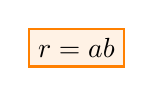
\begin{tikzpicture}[op/.style={rectangle,
        fill=orange!10, draw=orange}, thick]
      \node[op] {$r=a \mod b$};
    \end{tikzpicture}
  \end{lstlisting}
\end{Frame}

\begin{Frame}[fragile]{Knoten haben Stile.}{Entscheidungen}
  \tikzexample{[cn/.style={diamond, aspect=2, inner sep=2pt, fill=red!10, draw=red}, thick]
    \node[cn] {$b=0?$};
  }

  \xxx

  \begin{lstlisting}[gobble=4]
    \begin{tikzpicture}[cn/.style={diamond,
        aspect=2, inner sep=2pt,
        fill=red!10, draw=red}, thick]
      \node[cn] {$b=0?$};
    \end{tikzpicture}
  \end{lstlisting}
\end{Frame}

\begin{Frame}[t,fragile]{Knoten haben Namen.}
  \xxx\xxx
  \begin{columns}[T]
    \column{30mm}
      \tikzexample[left]{[io/.style={trapezium, trapezium left angle=70, trapezium right angle=110, fill=magenta!10, draw=magenta},
        op/.style={rectangle, fill=orange!10, draw=orange},
        cn/.style={diamond, aspect=2, inner sep=2pt, fill=red!10, draw=red}, thick]
        \node[io] at (0,4) (in) {Eingabe $a,b$};
        \node[op] at (0,3) (div) {$r=a \mod b$};
        \node[op] at (0,2) (set) {$a=b,\ b=r$};
        \node[cn] at (0,1) (cond) {$b=0?$};
        \node[io] at (0,0) (out) {Ausgabe $a$};
      }
    \column{55mm}
      \xxx
      \begin{lstlisting}[gobble=8]
        \node[io] at (0,4)
          (in) {Eingabe $a,b$};
        \node[op] at (0,3)
          (div) {$r=a \mod b$};
        \node[op] at (0,2)
          (set) {$a=b,\ b=r$};
        \node[cn] at (0,1)
          (cond) {$b=0?$};
        \node[io] at (0,0)
          (out) {Ausgabe $a$};
      \end{lstlisting}
  \end{columns}
\end{Frame}

\begin{Frame}[t,fragile]{Knoten relativ positionieren}
  \xxx\xxx
  \begin{columns}[T]
    \column{30mm}
      \tikzexample[left]{[io/.style={trapezium, trapezium left angle=70, trapezium right angle=110, fill=magenta!10, draw=magenta},
        op/.style={rectangle, fill=orange!10, draw=orange},
        cn/.style={diamond, aspect=2, inner sep=2pt, fill=red!10, draw=red}, thick, node distance=5mm]
        \node[io] (in) {Eingabe $a,b$};
        \node[op, below=of in] (div) {$r=a \mod b$};
        \node[op, below=of div] (set) {$a=b,\ b=r$};
        \node[cn, below=of set] (cond) {$b=0?$};
        \node[io, below=of cond] (out) {Ausgabe $a$};
      }
    \column{55mm}
      \xxx
      \begin{lstlisting}[gobble=8]
        \node[io]
          (in) {Eingabe $a,b$};
        \node[op, below=of in]
          (div) {$r=a \mod b$};
        \node[op, below=of div]
          (set) {$a=b,\ b=r$};
        \node[cn, below=of set]
          (cond) {$b=0?$};
        \node[io, below=of cond]
          (out) {Ausgabe $a$};
      \end{lstlisting}
  \end{columns}
\end{Frame}

\begin{Frame}[t,fragile]{Kanten}
  \xxx\xxx
  \begin{columns}[T]
    \column{30mm}
      \tikzexample[left]{[io/.style={trapezium, trapezium left angle=70, trapezium right angle=110, fill=magenta!10, draw=magenta},
        op/.style={rectangle, fill=orange!10, draw=orange},
        cn/.style={diamond, aspect=2, inner sep=2pt, fill=red!10, draw=red}, thick, node distance=5mm]
        \node[io] (in) {Eingabe $a,b$};
        \node[op, below=of in] (div) {$r=a \mod b$};
        \node[op, below=of div] (set) {$a=b,\ b=r$};
        \node[cn, below=of set] (cond) {$b=0?$};
        \node[io, below=of cond] (out) {Ausgabe $a$};
        %
        \path[->]
          (in) edge (div)
          (div) edge (set)
          (set) edge (cond)
          (cond) edge (out);
      }
    \column{55mm}
      \xxx
      \begin{lstlisting}[gobble=8]
        \path[->]
          (in) edge (div)
          (div) edge (set)
          (set) edge (cond)
          (cond) edge (out);
      \end{lstlisting}
  \end{columns}
\end{Frame}

\begin{Frame}[t,fragile]{Ein Pfad um die Ecke}
  \xxx\xxx
  \begin{columns}[T]
    \column{35mm}
      \tikzexample[left]{[io/.style={trapezium, trapezium left angle=70, trapezium right angle=110, fill=magenta!10, draw=magenta},
        op/.style={rectangle, fill=orange!10, draw=orange},
        cn/.style={diamond, aspect=2, inner sep=2pt, fill=red!10, draw=red}, thick, node distance=5mm]
        \node[io] (in) {Eingabe $a,b$};
        \node[op, below=of in] (div) {$r=a \mod b$};
        \node[op, below=of div] (set) {$a=b,\ b=r$};
        \node[cn, below=of set] (cond) {$b=0?$};
        \node[io, below=of cond] (out) {Ausgabe $a$};
        %
        \path[->]
          (in) edge (div)
          (div) edge (set)
          (set) edge (cond)
          (cond) edge (out);
        \draw[->] (cond) -- ++(1.5,0) |- (div);
      }
    \column{50mm}
      \xxx
      \begin{lstlisting}[gobble=8]
        \draw[->]
          (cond) -- ++(1.5,0)
                 |- (div);
      \end{lstlisting}
  \end{columns}
\end{Frame}

\begin{Frame}[t,fragile]{Beschriftete Kanten}{\texttt{examples/knoten.tex}}
  \xxx\xxx
  \begin{columns}[T]
    \column{35mm}
      \tikzexample[left]{[io/.style={trapezium, trapezium left angle=70, trapezium right angle=110, fill=magenta!10, draw=magenta},
        op/.style={rectangle, fill=orange!10, draw=orange},
        cn/.style={diamond, aspect=2, inner sep=2pt, fill=red!10, draw=red}, thick, node distance=5mm]
        \node[io] (in) {Eingabe $a,b$};
        \node[op, below=of in] (div) {$r=a \mod b$};
        \node[op, below=of div] (set) {$a=b,\ b=r$};
        \node[cn, below=of set] (cond) {$b=0?$};
        \node[io, below=of cond] (out) {Ausgabe $a$};
        %
        \path[->]
          (in) edge (div)
          (div) edge (set)
          (set) edge (cond)
          (cond) edge node[right] {Ja} (out);
        \draw[->] (cond) -- node[below] {Nein} ++(1.5,0) |- (div);
      }
    \column{50mm}
      \xxx
      \begin{lstlisting}[gobble=8]
        \path[->]
          (cond) edge
            node[right] {Ja}
              (out);
        \draw[->] (cond) --
          node[below] {Nein}
            ++(1.5,0) |- (div);
      \end{lstlisting}
  \end{columns}
\end{Frame}

\subsection{Automaten}

\begin{Frame}[fragile]{Automaten}
  \tikzexample{[auto, thick]
    \node[initial,state] (q0) {$q_0$};
    \visible<2->{\node[state, right=of q0] (q1) {$q_1$};}
    \visible<3->{\node[state, accepting, right=of q1] (q2) {$q_2$};}
    \visible<2->{\path
      (q0) edge[->] node {0} (q1)
      (q1) edge[->, loop above] node {0} ();}
    \visible<3->{\path
      (q1) edge[->, bend left] node {1} (q2)
      (q2) edge[->, bend left] node {0} (q1);}
  }

  \xxx

  \begin{lstlisting}[gobble=4,escapechar=\%]
    \tikz[auto, thick]{
      %\pause[1]%\node[initial, state] (q0) {$q_0$};            %\onslide%
      %\pause[2]%\node[state, right=of q0] (q1) {$q_1$};        %\onslide%
      %\pause[3]%\node[state, accepting, right=of q1]           %\onslide%
      %\pause[3]%  (q2) {$q_2$};                                %\onslide%
      %\pause[2]%\path (q0) edge[->] node {0} (q1)              %\onslide%
      %\pause[2]%      (q1) edge[->, loop above] node {0} ()    %\onslide%
      %\pause[3]%           edge[->, bend left] node {1} (q2)   %\onslide%
      %\pause[3]%      (q2) edge[->, bend left] node {0} (q1)%\pause[2]%;%\onslide%}
  \end{lstlisting}
\end{Frame}

\subsection{Bäume}

\begin{Frame}[fragile]{Bäume}{\texttt{examples/baum.tex}}
  \begin{columns}
    \column{42mm}
      \tikzexample[left]{[
        every node/.style={draw,circle,inner sep=0pt,minimum width=15pt},%
        edge from parent/.style={},%
        level/.style={sibling distance=20mm/#1},%
        level distance=10mm, thick]
        \node[coordinate] (root) {}
          child { child child }
          child { child child };
        %
        \node at (root) (a) {a};
        \visible<2->{\node at (root-1) (b) {b};}
        \visible<4->{\node at (root-2) (e) {e};}
        \visible<3->{\node at (root-1-1) (c) {c};}
        \visible<3->{\node at (root-1-2) (d) {d};}
        \visible<5->{\node at (root-2-1) (f) {f};}
        \visible<5->{\node at (root-2-2) (g) {g};}
        \visible<2->{\path (a) edge (b);}
        \visible<4->{\path (a) edge (e);}
        \visible<3->{\path (b) edge (c)
                       edge (d);}
        \visible<5->{\path (e) edge (f)
                       edge (g);}
      }

    \column{52mm}

    \begin{lstlisting}[gobble=6,escapechar=\%]
      %\pause[1]%\node {a}                %\onslide%
      %\pause[2]%  child { node {b}       %\onslide%
      %\pause[3]%    child { node {c} }   %\onslide%
      %\pause[3]%    child { node {d} }   %\onslide%
      %\pause[2]%  }                      %\onslide%
      %\pause[4]%  child { node {e}       %\onslide%
      %\pause[5]%    child { node {f} }   %\onslide%
      %\pause[5]%    child { node {g} }   %\onslide%
      %\pause[4]%  }%\onslide%;
    \end{lstlisting}
  \end{columns}
\end{Frame}



\malte
\beamersection{Fortgeschrittene Verwendung}

\subsection{Funktionen plotten}

\begin{Frame}{Beispiel eines Funktionsplots}{\lstinline|examples/funktionen.tex|}
  \tikzexample{[domain=0:5]
    \draw[very thin,gray] (0,-1.4) grid (4.9,3.4);
    \draw[->] (0,0) -- (5.2,0) node[right] {$x$};
    \draw[->] (0,-1.5) -- (0,3.5) node[above] {$f(x)$};
    %
    \foreach \x in {1,...,4}
      \draw[xshift=\x cm] (0,2pt) -- (0,-2pt) node[below,fill=tikzexample] {$\x$};
    \foreach \y in {-1,...,3}
      \draw[yshift=\y cm] (2pt,0) -- (-2pt,0) node[left,fill=tikzexample] {$\y$};
    %
    \draw[red]    plot (\x,\x/3)         node[right] {$f(x) = \frac{x}{3}$};
    \draw[blue]   plot (\x,{sin(\x r)})  node[right] {$f(x) = \sin x$};
    \draw[orange] plot (\x,{exp(\x)/50}) node[right] {$f(x) = \frac{e^x}{50}$};
  }
\end{Frame}

\begin{Frame}[fragile]{Funktionen plotten}
  \tikzexample{
    \draw[blue,domain=0:5] plot (\x,{sin(\x r)});
    \draw[orange,domain=0:4] plot (\x,{exp(\x)/50});
  }

  \xxx

  \begin{lstlisting}[gobble=4,moretexcs={x}]
    \draw[blue,domain=0:5] plot (\x,{sin(\x r)});
    \draw[orange,domain=0:4] plot (\x,{exp(\x)/50});
  \end{lstlisting}
\end{Frame}

\begin{Frame}[fragile]{Koordinatensystem}
  \tikzexample{
    \draw[very thin,gray] (0,-1.4) grid (4.9,1.4);
    \draw[->] (0,0) -- (5.2,0) node[right] {$x$};
    \draw[->] (0,-1.5) -- (0,1.5) node[above] {$f(x)$};
    %
    \draw[blue,domain=0:5] plot (\x,{sin(\x r)});
    \draw[orange,domain=0:4] plot (\x,{exp(\x)/50});
  }

  \xxx

  \begin{lstlisting}[gobble=4]
    \draw[very thin,gray] (0,-1.4) grid (4.9,1.4);
    \draw[->] (0,0) -- (5.2,0) node[right] {$x$};
    \draw[->] (0,-1.5) -- (0,1.5) node[above]
      {$f(x)$};
  \end{lstlisting}
\end{Frame}

\begin{Frame}[fragile]{Beschriftung der Achsen}
  \tikzexample{
    \draw[very thin,gray] (0,-1.4) grid (4.9,1.4);
    \draw[->] (0,0) -- (5.2,0) node[right] {$x$};
    \draw[->] (0,-1.5) -- (0,1.5) node[above] {$f(x)$};
    %
    \foreach \x in {1,...,4}
      \draw[xshift=\x cm] (0,2pt) -- (0,-2pt) node[below,fill=tikzexample] {$\x$};
    \foreach \y in {-1,...,1}
      \draw[yshift=\y cm] (2pt,0) -- (-2pt,0) node[left,fill=tikzexample] {$\y$};
    %
    \draw[blue,domain=0:5] plot (\x,{sin(\x r)});
    \draw[orange,domain=0:4] plot (\x,{exp(\x)/50});
  }

  \xxx

  \begin{lstlisting}[gobble=4]
    \foreach \x in {1,...,4}
      \draw[xshift=\x cm] (0,2pt) -- (0,-2pt)
        node[below,fill=white] {$\x$};
    \foreach \y in {-1,...,1}
      \draw[yshift=\y cm] (2pt,0) -- (-2pt,0)
        node[left,fill=white] {$\y$};
  \end{lstlisting}
\end{Frame}

\begin{Frame}[fragile]{Beschriftung der Graphen}
  \tikzexample{
    \draw[very thin,gray] (0,-1.4) grid (4.9,1.4);
    \draw[->] (0,0) -- (5.2,0) node[right] {$x$};
    \draw[->] (0,-1.5) -- (0,1.5) node[above] {$f(x)$};
    %
    \foreach \x in {1,...,4}
      \draw[xshift=\x cm] (0,2pt) -- (0,-2pt) node[below,fill=tikzexample] {$\x$};
    \foreach \y in {-1,...,1}
      \draw[yshift=\y cm] (2pt,0) -- (-2pt,0) node[left,fill=tikzexample] {$\y$};
    %
    \draw[blue,domain=0:5] plot (\x,{sin(\x r)}) node[right] {$f(x) = \sin x$};
    \draw[orange,domain=0:4] plot (\x,{exp(\x)/50}) node[right, fill=tikzexample] {$f(x) = \frac{e^x}{50}$};
  }

  \xxx

  \begin{lstlisting}[gobble=4, moretexcs={x}]
    \draw[blue,domain=0:5] plot (\x,{sin(\x r)})
      node[right] {$f(x) = \sin x$};
    \draw[orange,domain=0:4] plot (\x,{exp(\x)/50})
      node[right, fill=white]
        {$f(x) = \frac{e^x}{50}$};
  \end{lstlisting}
\end{Frame}

\subsection{Overlays mit \beamer}

\begin{Frame}{Beispiel von Overlays in Grafiken}{\lstinline|examples/tikz-overlays.tex|}
  \tikzexample{[dot/.style={circle,minimum width=5mm,fill=red},
      box/.style={draw, rectangle, inner sep=5mm},
      node distance=4mm and 18mm, thick]
    \uncover<2->{\node[dot] (n1) {};}
    \uncover<3->{\node[dot, right=of n1] (n2) {};}
    \uncover<4->{\node[dot, right=of n2] (n3) {};}
    \uncover<5->{\node[dot, below=of n1] (n4) {};}
    \uncover<6->{\node[dot, below=of n2] (n5) {};}
    \uncover<7->{\node[dot, below=of n3] (n6) {};}
    \node[box, fit=(n1) (n4)] (b1) {};
    \node[box, fit=(n2) (n5)] (b2) {};
    \node[box, fit=(n3) (n6)] (b3) {};
    \node[dot, below=8mm of b1.south west, anchor=west] (r1) {};
    \uncover<1-6>{\node[dot, right=4mm of r1] (r2) {};}
    \uncover<1-5>{\node[dot, right=4mm of r2] (r3) {};}
    \uncover<1-4>{\node[dot, right=4mm of r3] (r4) {};}
    \uncover<1-3>{\node[dot, right=4mm of r4] (r5) {};}
    \uncover<1-2>{\node[dot, right=4mm of r5] (r6) {};}
    \uncover<1>{\node[dot, right=4mm of r6] (r7) {};}
    \node[above=of b2] {$7 \textrm{ mod } 3 = \alt<7>{\alert{1}}{?}$};
  }
\end{Frame}

\begin{Frame}[fragile]{Stile}
  \tikzexample{[dot/.style={circle,minimum width=5mm,fill=red},
      box/.style={draw, rectangle, inner sep=5mm},
      node distance=4mm and 18mm, thick]
    \node[dot] (n1) {};
    \node[box, fit=(n1)] (b1) {};
  }

  \xxx

  \begin{lstlisting}[gobble=4]
    \begin{tikzpicture}[
        dot/.style={circle, minimum width=5mm,
          fill=red},
        box/.style={draw, rectangle,
          inner sep=5mm},
        node distance=4mm and 18mm, thick]
      \node[dot] (n1) {};
      \node[box, fit=(n1)] (b1) {};
    \end{tikzpicture}
  \end{lstlisting}
\end{Frame}

\begin{Frame}[fragile]{Positionierung}
  \begin{lstlisting}[gobble=4]
    \node[dot] (n1) {};
    \node[dot, right=of n1] (n2) {};
    \node[dot, below=of n1] (n4) {};
    % n3, n5, n6
    \node[box, fit=(n1) (n4)] (b1) {};
    % b2, b3
    \node[dot, below=8mm of b1.south west,
      anchor=west] (r1) {};
    % r2, r3, r4, r5, r6
    \node[dot, right=4mm of r6] (r7) {};
  \end{lstlisting}
\end{Frame}

\begin{Frame}[fragile]{Overlays}
  \begin{lstlisting}[gobble=4]
    \uncover<2->{\node[...] (n1) {};}
    % n2, n3, n4, n5
    \uncover<7->{\node[...] (n6) {};}
    \node[box, fit=(n1) (n4)] (b1) {};
    % b2, b3
    \node[dot, below=8mm of b1.south west,
      anchor=west] (r1) {};
    \uncover<1-6>{\node[...] (r2) {};}
    % r3, r4, r5, r6
    \uncover<1>{\node[...] (r7) {};}
  \end{lstlisting}
\end{Frame}

\subsection{Showcase}

\begin{Frame}[shrink]{Computer science mindmap}{Autor: Till Tantau}
  \begin{tikzpicture}
    \path[mindmap,concept color=black,text=white]
      node[concept] {Computer Science}
      [clockwise from=0]
      child[concept color=green!50!black] {
        node[concept] {practical}
        [clockwise from=90]
        child { node[concept] {algorithms} }
        child { node[concept] {data structures} }
        child { node[concept] {pro\-gramming languages} }
        child { node[concept] {software engineer\-ing} }
      }
      child[concept color=blue] {
        node[concept] {applied}
        [clockwise from=-30]
        child { node[concept] {databases} }
        child { node[concept] {WWW} }
      }
      child[concept color=red] { node[concept] {technical} }
      child[concept color=orange] { node[concept] {theoretical} };
  \end{tikzpicture}
\end{Frame}

\begin{Frame}{A family tree}{Autor: Stefan Kottwitz}
  \begin{tikzpicture}[
    man/.style={rectangle,draw,fill=blue!20},
    woman/.style={rectangle,draw,fill=red!20,rounded corners=.8ex},
    grandchild/.style={grow=down,xshift=1em,anchor=west,
      edge from parent path={(\tikzparentnode.south) |- (\tikzchildnode.west)}},
    first/.style={level distance=6ex},
    second/.style={level distance=12ex},
    third/.style={level distance=18ex},
    level 1/.style={sibling distance=5em},thick]
      % Parents
      \coordinate
        child[grow=left] {node[man,anchor=east]{Jim}}
        child[grow=right] {node[woman,anchor=west]{Jane}}
        child[grow=down,level distance=0ex]
      [edge from parent fork down]
      % Children and grandchildren
      child{node[man] {Alfred}
        child[grandchild,first] {node[man]{Joe}}
        child[grandchild,second] {node[woman]{Heather}}
        child[grandchild,third] {node[woman] {Barbara}}}
      child{node[woman] {Berta}
        child[grandchild,first] {node[man]{Howard}}}
      child {node[man] {Charles}}
      child {node[woman]{Doris}
        child[grandchild,first] {node[man]{Nick}}
        child[grandchild,second] {node[woman]{Liz}}};
  \end{tikzpicture}
\end{Frame}

\begin{Frame}{Circuit libraries}{Autor: Till Tantau}
  \begin{tikzpicture}[rotate=-90,circuit ee IEC,x=3.25cm,y=2.25cm]
    %  Let us start with some contacts:
    \foreach \contact/\y in {3/3.5,4/4.5,5/5.5}
    {
      \node [contact] (left contact \contact) at (0,\y) {};
      \node [contact] (right contact \contact) at (1,\y) {};
    }
    \draw (right contact 3)
       -- (right contact 4) -- (right contact 5);
    \draw (left contact 3) -- ++(down:.3) node[left] {\dots};
    \draw (right contact 3) -- ++(down:.3) node[left] {\dots};
    \draw (left contact 3) to [current direction'={near start,info=$\iota$},
                               resistor={near end,info={$R=4\ \Omega$}}]
                           (right contact 3);
    \draw (left contact 4) to [voltage source={near start,
                                               direction info={<-,info={\textrm{8\ V}}}},
                               resistor={info={$2\ \Omega$},near end}] (right contact 4);
    \draw (left contact 3) to [resistor={info={$1\ \Omega$}}] (left contact 4);
    \draw (left contact 4) to [resistor={info={$3\ \Omega$}}] (left contact 5);
    \draw (left contact 5) to [resistor={info={$4\ \Omega$}}] (right contact 5);
    \draw (left contact 5) to [diode] ++(up:1)
                           to [voltage source={near start,
                                               direction info={info={\textrm{3\ V}}}},
                               resistor={near end,info={$3\ \Omega$}}] ++(right:1)
                           to (right contact 5);
  \end{tikzpicture}
\end{Frame}

\begin{Frame}[fragile,shrink]{BER measurement on fibre optical system}{Author: Jose Luis Diaz}
  \only<presentation>{\vspace*{2.5cm}}
  \only<article>{\sideways}
  \begin{tikzpicture}
    % Define a macro to draw the filter symbol
    \newcommand{\filterSS}[1]{\node (#1){};  % This empty node draws the box. 
       % Then we draw the inner curves
       \draw[line width=1pt] (-2mm,-4mm) to[in=200,out=20] (-2mm, 4mm) 
                             (0mm,-4mm) to[in=200,out=20] (0mm, 4mm) 
                             (2mm,-4mm) to[in=200,out=20] (2mm, 4mm); 
       }

    % Define a macro to draw the MOD symbol
    \newcommand{\MOD}[2]{\node (#1) {#2}; % The box with the text inside. Then draw the polygon around the text
      \draw[line width=1pt,sharp corners](-0.75cm,0cm)--(-0.35cm,0.25cm)--
           (0.35cm, 0.25cm)--(0.75cm, 0cm)--(0.35cm, -0.25cm)--(-0.35cm, -0.25cm) -- cycle; 
      }

    % Define a macro to draw the Polariser symbol
    \newcommand{\Polaris}[1]{\node[coordinate] (#1) {}; % Node of type coordinate is a simple point 
         % Now draw the three circles
         \draw[line width=1pt] (0mm, -2mm)  circle (2mm) 
                               (-2mm,2mm)  circle (2mm)
                               (2mm, 2mm)  circle (2mm);}

    % Place all element in a matrix of nodes, called m
    % By default all nodes are rectangles with round corners
    % but some special sytles are defined also
    \matrix (m) [
      column sep=5mm,
      row sep=1cm,
      nodes={draw, % General options for all nodes
        line width=1pt,
        anchor=center, 
        text centered,
        rounded corners,
        minimum width=1.5cm, minimum height=8mm
      }, 
      % Define styles for some special nodes
      right iso/.style={isosceles triangle,scale=0.5,sharp corners, anchor=center, xshift=-4mm},
      left iso/.style={right iso, rotate=180, xshift=-8mm},
      txt/.style={text width=1.5cm,anchor=center},
      ellip/.style={ellipse,scale=0.5},
      empty/.style={draw=none}
      ]
    {
    % First row of symbols (mostly empty, only the power meter at the right end)
      % empty
    & % empty
    & % empty
    & % empty
    & % empty
    & % empty
    & \node[txt] (top power meter) {Power Meter};
    \\

    % Second row of symbols
      \node (laser) {Laser};
    & \MOD{mod}{MOD} 
    & \node[right iso] (iso 1) {};
    & \node (top soa) {SOA};
    & \filterSS{top filter} 
    & \node (top voa) {VOA};
    & \node[ellip] (top connector) {};
    & \node[coordinate, xshift=-1cm] (top right) {};
    \\
    % Third row of symbols
    & \node (mid voa) {VOA};
    & \filterSS{mid filter}  
    & \node[left iso] (iso 2) {};
    & \node[draw=orange!80!white, ultra thick] (qdsoa) {\textbf{QDSOA}};
    & \node[left iso] (iso 3) {};
    & \Polaris{Polaris} 
    & % (no symbol here, only a point to draw the path)
      \node[coordinate, xshift=-1cm] (mid right) {};
    \\
    % Fourth row of symbols
      \node[txt] (low power meter) {Power Meter};
    & \node[ellip] (low ellip) {};
    & \node[right iso] (iso 4) {};
    & \node (low soa) {SOA};
    & \node[right iso] (iso 5) {};
    & \filterSS{low filter} 
    & \node (rx) {Rx};
    & \node[txt] (error detector) {Error\\Detector};
    \\
    };  % End of matrix

    % Now, connect all nodes in a chain.
    % The names of the nodes are automatically generated in the previous matrix. Since the
    % matrix was named ``m'', all nodes have the name m-row-column
    { [start chain,every on chain/.style={join}, every join/.style={line width=1pt}]
      \chainin (laser);
      \chainin (mod);
      \chainin (iso 1);
      \chainin (top soa);
      \chainin (top filter);
      \chainin (top voa);
      % Connect to the power meter, and put a label saying 10%
      \path[line width=1pt] (top power meter) edge node [right] {$10\%$} (top connector);
      \chainin (top connector);
      \chainin (top right);
      % Draw the label saying 90%
      \path (top right) edge node [right] {$90\%$} (mid right) ;
      \chainin (mid right);
      \chainin (Polaris);
      \chainin (iso 3);
      \chainin (qdsoa);
      \chainin (iso 2);
      \chainin (mid filter);
      \chainin (mid voa);
      % Connect to the power meter, and put a label saying 10%
      \path[line width=1pt] (low power meter) edge node [above] {$10\%$} (low ellip);
      \chainin (low ellip);
      % Draw the label saying 90%
      \path (low ellip) edge node [below] {$90\%$} (iso 4) ;
      \chainin (iso 4);
      \chainin (low soa);
      \chainin (iso 5);
      \chainin (low filter);
      \chainin (rx);
      \chainin (error detector);
      };
    % Finally, put some text above some symbols
    \draw (iso 1.left side) node[above, inner sep=5mm] {Isolator};
    \draw (top filter.north) node[above, inner sep=3mm] {Filter};
    \draw (Polaris) node[above, inner sep=6mm, text centered, text width=2cm] {Polarisation\\controller};

    % The big arrow over the MOD symbol is a bit laborious
    \node[yshift=2mm] (MOD arrow) at (mod.north) [anchor=east,single arrow, draw,line width=1pt, 
                  rotate=-90, minimum height=7mm, minimum width=1.3cm, 
                  single arrow head extend=1.2mm, single arrow tip angle=120] {};
    % The text above the arrow (the starting of the arrow is at west in the arrow shape, even if the
    % arrow was rotated and it lies now at top)
    \node (MOD text) at (MOD arrow.west) [above, inner sep=2mm] {10Gb/s PRBS};

    % Define the style for the blue dotted boxes
    \tikzset{blue dotted/.style={draw=blue!50!white, line width=1pt,
                                 dash pattern=on 1pt off 4pt on 6pt off 4pt,
                                  inner sep=4mm, rectangle, rounded corners}};

    % Finally the blue dotted boxes are drawn as nodes fitted to other nodes
    \node (first dotted box) [blue dotted, 
                              fit = (MOD text) (laser) (top soa)] {};
    \node (second dotted box) [blue dotted,
                              fit = (low soa) (error detector)] {};

    % Since these boxes are nodes, it is easy to put text above or below them                          
    \node at (first dotted box.north) [above, inner sep=3mm] {\textbf{Transmitter}};
    \node at (second dotted box.south) [below, inner sep=3mm] {\textbf{Receiver}};
  \end{tikzpicture}
  \only<presentation>{\vspace*{2.5cm}}
  \only<article>{\endsideways}
\end{Frame}

\begin{Frame}[fragile]{Map of a HiSPARC detector}{Autor: David Fokkema}
  \newcommand{\hisparcbox}[1]{%
    \path[hisparc,#1]
        (-.4, .7) .. controls (0, .75) ..  (.4, .7) --
        (.35, -1.7) ..  controls(0, -1.72) ..  (-.35, -1.7) -- cycle;
  }
  \begin{tikzpicture}
    [ x=.5mm, y=.5mm, scale=0.6,
      font={\sffamily},
      station/.style={fill=gray},
      hut/.style={fill=lightgray},
      cluster/.style={fill=yellow!30, rounded corners=2pt},
      road/.style={fill=blue!10},
      calorimeter/.style={fill=green!30},
      tracker/.style={fill=red!30},
      hisparc/.style={fill=red, rounded corners=.15pt},
      hisparcgps/.style={fill=red},
      axis/.style={gray,very thick,->,>=stealth'},
      ruler/.style={gray,|<->|,>=stealth'}
    ]
    % Clusters
    \foreach \i in {-1.5, -0.5, ..., 1.5} {
        \foreach \j in {-1.5, -0.5, ..., 1.5} {
            \path[cluster, shift={(\i * 52, \j * 52)}]
                (-22, -22) rectangle (22, 22);
        }
    }

    % Roads
    \foreach \i in {-1.5, -0.5, ..., 1.5} {
        \path[road, shift={(0, \i * 52 + 2)}]
            (-105, -1.5) rectangle (105, 1.5);
    }

    % Detector array
    \foreach \i in {-7.5, -6.5, ..., 7.5} {
        \foreach \j in {-7.5, -6.5, ..., 7.5} {
            \path[station, shift={(\i * 13, \j * 13)}]
                (-1.2, -1.2) rectangle (1.2, 1.2);
        }
    }
    % Two detectors are slightly displaced
    \path[station, shift={(-6.5, 23.5)}] (-1.2, -1.2) rectangle (1.2, 1.2);
    \path[station, shift={(6.5, 23.5)}] (-1.2, -1.2) rectangle (1.2, 1.2);

    % Electronic huts
    \foreach \i in {-1.5, -0.5, ..., 1.5} {
        \foreach \j in {-1.5, -0.5, ..., 1.5} {
            \path[hut, shift={(\i * 52, \j * 52 - 1.5)}]
                (-2.5, -1.2) rectangle (2.5, 1.2);
        }
    }

    % Central detector
    \fill[white] (-13, -13) rectangle (13, 21);
    \path[calorimeter, shift={(0, 5)}] (-10, -8) rectangle (10, 8);

    % Muon tracker
    \path[tracker, shift={(0, 4)}] (-2.7, 32.5) rectangle (2.7, 70.5);

    % HiSPARC station
    \hisparcbox{shift={(65.0, 15.05)}, rotate=180}
    \hisparcbox{shift={(65.0, 20.82)}, rotate=180}
    \hisparcbox{shift={(70.0, 23.71)}, rotate=-90}
    \hisparcbox{shift={(60.0, 23.71)}, rotate=90}
    \path[hisparcgps, shift={(65.0, 23.71)}] (0, 0) circle (.3);

    % Draw rulers
    \draw[ruler] (-97.5, -105) -- (97.5, -105)
        node[midway,below] {195\ m};
    \draw[ruler] (84.5, 105) -- (97.5, 105)
        node[midway,above] {13\ m};
    \draw[ruler] (-105, -97.5) -- (-105, 97.5)
        node[midway,above,sloped] {195\ m};
    \draw[ruler] (105, 84.5) -- (105, 97.5)
        node[midway,below,sloped] {13\ m};
  \end{tikzpicture}
\end{Frame}

\begin{Frame}[fragile]{Lipid vesicle}{Autor: Henrik Skov Midtiby}
  % Define decoration
  \pgfdeclaredecoration{lipidleaflet}{initial}
  {
    % Place as many segments as possible along the path to decorate
    % the minimum distance between two segments is set to 7 pt.
    \state{initial}[width=\pgfdecoratedpathlength/floor(\pgfdecoratedpathlength/7pt)]
    {
      % Draw the two acyl chains
      \pgfpathmoveto{\pgfpoint{-1pt}{0pt}}
      \pgfpathlineto{\pgfpoint{-1pt}{-10pt}}
      \pgfpathmoveto{\pgfpoint{1pt}{0pt}}
      \pgfpathlineto{\pgfpoint{1pt}{-10pt}}
      % Draw the head group
      \pgfpathmoveto{\pgfpoint{1pt}{0pt}}
      \pgfpathcircle{\pgfpoint{0pt}{2pt}}{2.5pt}
    }
    \state{final}
    {
      \pgfpathmoveto{\pgfpointdecoratedpathlast}
    }
  }

  % Draw a vesicle composed of two lipid layers
  \begin{tikzpicture}
  % Micelle
  \draw[decorate, decoration={lipidleaflet, mirror}] (0, 3) circle (0.6cm);
  \draw (0, 2) node {Micelle};

  % Inverted micelle
  \draw[decorate, decoration={lipidleaflet}] (0, 0) circle (0.45cm);
  \draw (0, -1) node {Inverted micelle};

  % Lipid bilayer
  \draw[decorate, decoration={lipidleaflet, mirror}]
    (-1, -2.8) -- (2, -2.8);
  \draw[decorate, decoration={lipidleaflet}]
    (-1, -2) -- (2, -2);
  \draw (0, -3.5) node {Lipid bilayer};

  % Vesicle
  \draw[decorate, decoration={lipidleaflet}] (5, 0.5) circle (2.5cm);
  \draw[decorate, decoration={lipidleaflet, mirror}] (5, 0.5) circle (3.3cm);
  \draw (5, -3.5) node {Vesicle};

  \end{tikzpicture}
\end{Frame}

\begin{Frame}{Daniell's pile}{Autor: Agustin E. Bolzan}
  \definecolor{copper}{cmyk}{0,0.9,0.9,0.2}
  \colorlet{lightgray}{black!25}
  \colorlet{darkgray}{black!75}
  \begin{tikzpicture}[scale=1.5]
    % Draw back of vessel 1
    \draw (0,0) to [controls=+(90:0.5) and +(90:0.5)] (2,0);
    \draw[fill=blue!60, fill opacity=0.5] (0,-0.5) to
        [controls=+(90:0.5) and +(90:0.5)] (2,-0.5);

    % Draw back of vessel 2
    \draw (3.5,0) to [controls=+(90:0.5) and +(90:0.5)] (5.5,0);
    \draw[fill=lightgray, fill opacity=0.5] (3.5,-0.5) to [controls=+(90:0.5)
        and +(90:0.5)] (5.5,-0.5);

    % Draw copper electrode
    \draw[fill=copper] (0.5,2) rectangle (1.5,-1);
    \draw (0,2.3) node {Cu};
    \draw (1,-1.75) node {\small{CuSO$_{4}$}};

    % Draw salt bridge

    \draw[line join=round, line width=10pt] (1.75,-1.75) -- (1.75,0.5) --
        (3.75, 0.5) -- (3.75,-1.75);
    \draw[line join=round, line width=5pt, color=gray!25] (1.75,-1.75) --
        (1.75,0.5) -- (3.75, 0.5) -- (3.75,-1.75);
    \draw (2.75,0.5) node {\tiny{KNO$_{3}$}};

    %Draw front of vessel 1

    \draw (0,0) .. controls +(-90:0.5) and +(-90:0.5) .. (2,0);
    \draw (0,0) .. controls +(-90:0.5) and +(-90:0.5) .. (2,0)
        -- (2,-0.5) .. controls +(-90:0.5) and +(-90:0.5) .. (0,-0.5) -- (0,0);

    %Second part

    \draw[fill=blue!60, fill opacity=0.5] (0,-0.5) .. controls +(-90:0.5)
    and +(-90:0.5) .. (2,-0.5);
    \draw[fill=blue!60, fill opacity=0.5] (0,-0.5) .. controls +(-90:0.5)
    and +(-90:0.5) .. (2,-0.5)
        -- (2,-2) .. controls +(-90:0.5) and +(-90:0.5) .. (0,-2) -- (0,-0.5);

    % draw voltmeter

    \draw[line join=round, thick] (1,2) -- (1,2.5) -- (4.5,2.5) -- (4.5,2);
    \draw (2.75,2.5) node [circle, draw, fill=red!30] {V};

    %Draw back of vessel 2

    %Draw electrode

    \draw[fill=darkgray] (4,2) rectangle (5,-1);
    \draw (5.5,2.3) node {Zn};
    \draw (4.5,-1.75) node {\small{ZnSO$_{4}$}};

    % Draw front of vessel 2
    % part 1
    \draw (3.5,0) .. controls +(-90:0.5) and +(-90:0.5) .. (5.5,0);
    \draw (3.5,0) .. controls +(-90:0.5) and +(-90:0.5) .. (5.5,0)
        -- (5.5,-0.5) .. controls +(-90:0.5) and +(-90:0.5)
        .. (3.5,-0.5) -- (3.5,0);
    % part 2
    \draw[fill=lightgray, fill opacity=0.5] (3.5,-0.5) .. controls +(-90:0.5)
    and +(-90:0.5) .. (5.5,-0.5);
    \draw[fill=lightgray, fill opacity=0.5] (3.5,-0.5) .. controls +(-90:0.5)
        and +(-90:0.5) .. (5.5,-0.5) --
        (5.5,-2) .. controls +(-90:0.5) and +(-90:0.5)
        .. (3.5,-2) -- (3.5,-0.5);
  \end{tikzpicture}
\end{Frame}

\begin{Frame}{Membrane-like surface}{Autor: Yotam Avital}
  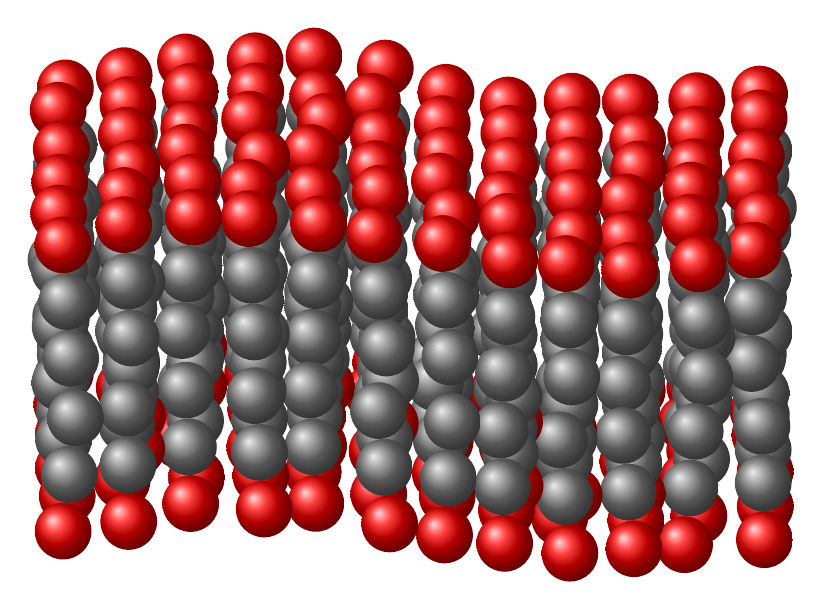
\begin{tikzpicture}[scale=0.8]
    \def\nuPi{3.1459265}
    \foreach \i in {11,10,...,0}{% This one doesn't matter
      \foreach \j in {5,4,...,0}{% This will crate a membrane
                                 % with the front lipids visible
        % top layer
        \pgfmathsetmacro{\dx}{rand*0.1}% A random variance in the x coordinate
        \pgfmathsetmacro{\dy}{rand*0.1}% A random variance in the y coordinate,
                                       % gives a hight fill to the lipid
        \pgfmathsetmacro{\rot}{rand*0.1}% A random variance in the
                                        % molecule orientation
        \shade[ball color=red] ({\i+\dx+\rot},{0.5*\j+\dy+0.4*sin(\i*\nuPi*10)}) circle(0.45);
        \shade[ball color=gray] (\i+\dx,{0.5*\j+\dy+0.4*sin(\i*\nuPi*10)-0.9}) circle(0.45);
        \shade[ball color=gray] (\i+\dx-\rot,{0.5*\j+\dy+0.4*sin(\i*\nuPi*10)-1.8}) circle(0.45);
        % bottom layer
        \pgfmathsetmacro{\dx}{rand*0.1}
        \pgfmathsetmacro{\dy}{rand*0.1}
        \pgfmathsetmacro{\rot}{rand*0.1}
        \shade[ball color=gray] (\i+\dx+\rot,{0.5*\j+\dy+0.4*sin(\i*\nuPi*10)-2.8}) circle(0.45);
        \shade[ball color=gray] (\i+\dx,{0.5*\j+\dy+0.4*sin(\i*\nuPi*10)-3.7}) circle(0.45);
        \shade[ball color=red] (\i+\dx-\rot,{0.5*\j+\dy+0.4*sin(\i*\nuPi*10)-4.6}) circle(0.45);
      }
    }
  \end{tikzpicture}
\end{Frame}

\begin{Frame}[fragile]{Christmas fractal tree}{Autor: Andrew Stacey}
  \tikzset{
    tinsel/.style={
      #1,
      rounded corners=10mm,
      ultra thin,
      decorate,
      decoration={
        snake,
        amplitude=.1mm,
        segment length=10,
      }
    },
    baubles/.style={
      decorate,
      decoration={
        markings,
        mark=between positions .3 and 1 step 2cm
        with
        {
          \pgfmathsetmacro{\brad}{2 + .5 * rand}
          \path[shading=ball,ball color=#1] (0,0) circle[radius=\brad mm];
        }
      }
    },
    lights/.style={
      decorate,
      decoration={
        markings,
        mark=between positions 0 and 1 step 1cm
        with
        {
          \pgfmathsetmacro{\tint}{100*rnd}
          \node[rotate=90,dart,shading=ball,inner sep=1pt,ball color=red!\tint!yellow] {};
        }
      }
    }
  }
  \qquad
  \begin{tikzpicture}[scale=0.8]
    \coordinate (star) at (0,-1);
    \path (star) +(-50:7) coordinate (rhs) +(-130:7) coordinate (lhs);
    \draw[brown!50!black,line width=5mm,line cap=round] (star) ++(-90:6.8) -- ++(0,-1) coordinate (base);
    \node[scale=-1,trapezium,fill=black,minimum size=1cm] at (base) {};
    \foreach \height/\colour in {%
      .2/blue,
      .4/yellow,
      .6/red,
      .8/orange,
      1/pink%
    } {
      \draw[tinsel=\colour] ($(star)!\height!(lhs)$) to[bend right] ($(star)!\height!(rhs)$);
    }
    \path (star);
    \pgfgetlastxy{\starx}{\stary}
    \begin{scope}[xshift=\starx,yshift=\stary,yshift=-7cm]
    \draw[color=green!50!black, l-system={rule set={S -> [+++G][---G]TS,  G -> +H[-G]L, H -> -G[+H]L, T -> TL, L -> [-FFF][+FFF]F}, step=4pt, angle=18, axiom=+++++SLFFF, order=11}] lindenmayer system -- cycle;
    \end{scope}
    \foreach \height/\colour in {%
      .1/pink,
      .3/red,
      .5/yellow,
      .7/blue,
      .9/orange%
    } {
      \draw[tinsel=\colour] ($(star)!\height!(lhs)$) to[bend right] ($(star)!\height!(rhs)$);
    }
    \foreach \height in {.15,.35,...,1} {
      \draw[lights] ($(star)!\height!(lhs)$) to[bend right] ($(star)!\height!(rhs)$);
    }
    \foreach \angle/\colour in {
      -50/red,
      -70/yellow,
      -90/blue,
      -110/pink,
      -130/purple%
    } {
      \draw[baubles=\colour] (star) -- ++(\angle:7);
    }
    \node[star,star point ratio=2.5,fill=yellow,minimum size=1cm] at (star) {};
  \end{tikzpicture}
\end{Frame}



\malte
\section*{Zusammenfassung}

\begin{frame}{Zusammenfassung}
  \begin{enumerate}
    \item \TikZ-Zeichnungen bestehen aus \alert{Pfaden}, die über \alert{Koordinaten} definiert werden.
    \item Fast alle scheamtischen Zeichnungen sind ein \alert{Graph}, bestehen also aus \alert{Knoten} und \alert{Kanten} und
      werden auch als solche in \TikZ\ gezeichnet.
    \item \TikZ\ ist sehr umfangreich und enthält \alert{sehr viele Bibliotheken}.
    \item Bei Problemen und Fragen \alert{lies die Anleitung!}
  \end{enumerate}
\end{frame}

\begin{Frame}{Zum Weiterlesen}
  \begin{mybib}
    \bibitem{Tantau4}
      Till Tantau.
      \newblock \emph{The \TikZ\ and \textsc{pgf} Packages},
      \newblock Manual for version 2.10,
      \newblock \alt<presentation>{\href{http://mirrors.ctan.org/graphics/pgf/base/doc/generic/pgf/pgfmanual.pdf}{\texttt{pgfmanual.pdf}}}{\url{http://mirrors.ctan.org/graphics/pgf/base/doc/generic/pgf/pgfmanual.pdf}}, Oktober 2010.

    \bibitem{Texample}
      Kjell Magne Fauske und Stefan Kottwitz.
      \newblock \emph{\TeX ample.net},
      \newblock ample resources for TeX users,
      \newblock \alt<presentation>{\href{http://www.texample.net/tikz/examples/}{\texttt{texample.net}}}{\url{http://www.texample.net/tikz/examples/}}.
  \end{mybib}
\end{Frame}



%% Begin Beamer talk
\malte

\label{chapter-beamer}
\chapter{Präsentationen mit \beamer}

\targets{
  \item \strut\beamer\ verwenden können.
  \item Vor- und Nachteile von \beamer\ kennen und einschätzen können, wann und wofür \beamer\ gut geeignet ist.
  \item Fortgeschrittene Anwendungsmöglichkeiten von \beamer\ kennen lernen.
}

\website

\jonny
\beamersection{Was ist \beamer?}

\subsection{Einleitung}

\begin{Frame}{Was ist \beamer?}
  \begin{itemize}
    \item \alert{Dokumentenklasse für \LaTeX} für die Erzeugung von Präsentationen.
      \only<article>{\newline(Diese Präsentation und das Skript wurden mit \beamer\ erzeugt.)}
    \item Keine eigene und \alert{keine graphische Anwendung}.
    \item \strut\beamer\ ist in \MiKTeX\ und \TeX\ Live enthalten.\newline
      (\alert{Es kann direkt losgehen}.)
  \end{itemize}
\end{Frame}

\mode
<article>

\begin{Frame}{Historie}
  \begin{description}
    \item[1998] Till Tantau erzeugt sich erste Makros für Präsentationen.
    \item[2003] Er verwendet die erste Version für seine Promotionsverteidigung.
    \item[2003] Veröffentlichung und Implementierung von vielen Benutzerwünschen.
    \item[2007] \beamer\ wird nicht weiter gepflegt.
    \item[2010] \beamer\ wird an Joseph Wright and Vedran Mileti\'c übergeben.
    \item[2014] Aktuelle Version 3.33 wird kontinuierlich weiter entwickelt.
  \end{description}
\end{Frame}

\mode
<all>

\begin{Frame}{Workflow}
  \lstset{language={}}
  \begin{enumerate}
    \item Normales \LaTeX-Dokument erzeugen.\\
      Dabei einige spezielle \beamer-Kommandos verwenden.
    \item \LaTeX-Dokument mit \lstinline-pdflatex- kompilieren.
    \item Ergebnis überprüfen und \LaTeX-Dokument anpassen.
  \end{enumerate}
\end{Frame}

\subsection{Eigenschaften}

\begin{Frame}{Funktionsweise von \beamer}
  \begin{itemize}
    \item Kompilieren wie jedes andere \LaTeX-Dokument auch.
    \item Normale \LaTeX-Kommandos funktionieren.
    \item Sinnvolles funktionales Aussehen von Vorträgen.
    \item Einfaches Ein- und Ausblenden von Seitenteilen.
    \item Automatische Gliederungen und Navigationsleisten.
    \item Präsentationen im PDF-Format können auf jedem Computer dargestellt werden.
  \end{itemize}
\end{Frame}

\begin{Frame}{\beamer\ vs. PowerPoint}
  \begin{zebratabular}{rcc}
    \headerrow Aspekte & \beamer\ & PowerPoint \\
    Erlernen ohne \LaTeX-Kenntnisse & \badmark\badmark & \goodmark \\
    Objekte frei positionieren & \badmark & \goodmark\goodmark \\
    Grafiken direkt erstellen & \badmark & \goodmark \\
    Einbinden von Multimedia & -- & \goodmark \\
    Arbeitsgeschwindigkeit Anfänger & -- & -- \\
    Arbeitsgeschwindigkeit Profi & \goodmark & \goodmark \\
    Erlernen mit \LaTeX-Kenntnissen & \goodmark & \goodmark \\
    Dokumentation & \goodmark & \goodmark \\
    Vorlagenqualität & \goodmark & -- \\
    Typographie & \goodmark & \badmark\badmark \\
    Konsistenz des Aussehens & \goodmark\goodmark & \badmark \\
    Visualisierung des Vortragsaufbaus & \goodmark\goodmark & \badmark \\
    Mathematische Formeln & \goodmark\goodmark & \badmark\badmark \\
    Quelltextdarstellung & \goodmark\goodmark & \badmark\badmark
  \end{zebratabular}
\end{Frame}


\beamersection{Verwendung von \beamer}

\begin{Frame}[fragile]{Beispiel}
  \begin{lstlisting}[gobble=4]
    \documentclass{beamer}

    \usepackage[utf8]{inputenc}
    \usepackage[T1]{fontenc}
    \usepackage{lmodern}
    \usepackage[ngerman]{babel}

    \begin{document}
      \begin{frame}{Funktionen von Beamer}
        Kompilieren wie jedes andere
        \LaTeX-Dokument auch.
      \end{frame}
    \end{document}
  \end{lstlisting}
\end{Frame}

\beamerexample{demo/beamer.pdf}

\subsection{Folien}

\begin{Frame}[fragile]{Folien}
  \begin{itemize}
    \item Ein \beamer-Dokument besteht aus mehreren Frames.
    \item Jeder Frame kann aus mehreren Slides bestehen.
    \item Die Umgebung \lstinline-frame- verarbeitet
      bis zu zwei Parameter in gescheiften Klammern \lstinline-{}-
    \item Der erste Parameter ist der Titel.
    \item Der zweite Parameter ist der Untertitel.
    \item Innerhalb der Umgebung \lstinline|frame| wird normaler \LaTeX-Code
      verwendet.
  \end{itemize}
\end{Frame}

\begin{Frame}[fragile]{Titelfolie}
  \begin{Block}{In der Präambel}
    \begin{lstlisting}[gobble=6,style=block]
      \title[Kurztitel]{%
        Lange Version des langen Titels}
      \subtitle{Ein langer Untertitel beschreibt
        alles noch etwas genauer.}
      \author[Thorn, Schmitz]{%
        Johannes Thorn \and Malte Schmitz}
      \date[KPT 2014]{Konferenz über
        Präsentationstechniken, 2014}
    \end{lstlisting}
  \end{Block}

  \begin{lstlisting}[gobble=4]
    \begin{frame}
      \maketitle
    \end{frame}
  \end{lstlisting}
\end{Frame}

\beamerexample{demo/beamer-titlepage.pdf}

\begin{Frame}[fragile]{Gliederung}
  \begin{itemize}
    \item Strukturbefehle außerhalb von \lstinline-frame-\\
      normal verwenden.
      \begin{itemize}
        \item ca. 3 Abschnitte mit \lstinline-\section-
        \item je max. 4 Unterabschnitte mit \lstinline-\subsection-
      \end{itemize}
    \item \lstinline-\tableofcontents- im \lstinline-frame- setzt das Inhaltsverzeichnis.
    \item Je nach Theme erscheinen \lstinline-\section- und
      \lstinline-\subsection- auch in Navigationsleisten.
    \item \lstinline-\section*- und \lstinline-\subsection*- erscheinen in
      Navigationsleisten aber nicht im Inhaltsverzeichnis.
  \end{itemize}
\end{Frame}

\subsection{Strukturelemente}

\begin{Frame}[fragile]{Listen, Tabellen und Grafiken}
  \begin{itemize}
    \item Listen mit \lstinline-itemize- und \lstinline-enumerate-,
    \item Tabellen mit \lstinline-tabular- und
    \item Grafiken mit \lstinline-\includegraphics- funktionieren wie immer in \LaTeX.
  \end{itemize}

  \xxx

  \begin{itemize}
    \item Eine Folie ist 128~mm $\times$ 96~mm groß.
    \item Zeilenumbruch \lstinline-\\- zum Ausrichten von Text sinnvoll.
  \end{itemize}
\end{Frame}

\begin{Frame}[fragile]{Formelsatz}
  \begin{itemize}
    \item Formelsatz wie immer in \LaTeX
    \item zum Beispiel \lstinline-$1+1=2$-\\
      oder \lstinline-\[1+1=2\]-
  \end{itemize}

  \xxx

  \begin{lstlisting}[gobble=4]
    % Formeln mit Serifen setzen
    \usefonttheme[onlymath]{serif}
  \end{lstlisting}
\end{Frame}

\begin{Frame}[fragile]{Blöcke}
  \begin{lstlisting}[gobble=4]
    \begin{block}{Überschrift}
      Dieser Text steht im normalen Block.
    \end{block}

    \begin{alertblock}{Achtung}
      Dieser Text steht im hervorgehobenen Block.
    \end{alertblock}

    \begin{exampleblock}{Beispiel}
      Dieser Text steht im Beispielblock.
    \end{exampleblock}
  \end{lstlisting}
\end{Frame}

\beamerexample{demo/beamer-struktur.pdf}

\begin{Frame}[fragile]{Theorem-Umgebungen}
  \begin{lstlisting}[gobble=4]
    \begin{Satz}[Sandhaufensatz]
      Es gibt keine Sandhaufen.
    \end{Satz}

    \begin{Beweis}
      \begin{enumerate}
        \item Ein Sandkorn ist kein Sandhaufen.
        \item Sandkörner werden durch Hinzufügen
          eines Sandkorns nicht zum Sandhaufen.
        \item Induktiv folgt die Aussage. \qedhere
      \end{enumerate}
    \end{Beweis}
  \end{lstlisting}
\end{Frame}

\beamerexample[2]{demo/beamer-struktur.pdf}

\begin{Frame}[fragile]{Spalten}
  \begin{lstlisting}[gobble=4]
    \begin{frame}{Spalten}
      \begin{columns}
        \begin{column}{5cm}
          Linke Spalte.
        \end{column}
        \begin{column}{5cm}
          Rechte Spalte.
        \end{column}
      \end{columns}
    \end{frame}
  \end{lstlisting}
\end{Frame}

\beamerexample[3]{demo/beamer-struktur.pdf}

\begin{Frame}[fragile]{Quelltext ist fragil.}
  \begin{Block}{In der Präambel}
    \begin{lstlisting}[style=block,gobble=6]
      \usepackage{listings}
      \lstset{%
        basicstyle=\ttfamily,%
        showstringspaces=false,%
        upquote=true}
      \usepackage{textcomp} % für upquote
    \end{lstlisting}
  \end{Block}

  \xxx

  \lstinputlisting{demo/beamer-listing-content.tex}
\end{Frame}

\beamerexample{demo/beamer-listing.pdf}

\subsection{Form}

\begin{Frame}[fragile]{Themes}
  \begin{description}[labelwidth=5em]
    \item[Theme]
      \begin{itemize}
        \item geladen durch \lstinline-\usetheme{name}- 
        \item bestimmt die \alert{allgemeine Form} der Präsentation
      \end{itemize}
    \item[Inner Theme]
      \begin{itemize}
        \item geladen durch \lstinline-\useinnertheme{name}- 
        \item bestimmt die \alert{Form des Folieninhalts}
      \end{itemize}
    \item[Outer Theme]
      \begin{itemize}
        \item geladen durch \lstinline-\useoutertheme{name}- 
        \item bestimmt die \alert{Form der Layoutelemente}
      \end{itemize}
    \item[Color Theme]
      \begin{itemize}
        \item geladen durch \lstinline-\usecolortheme{name}- 
        \item bestimmt die \alert{allgemeine Farbe} der Präsentation
      \end{itemize}
  \end{description}
\end{Frame}

\beamerexample[23]{demo/beamer-Boadilla.pdf}

\beamerexample[23]{demo/beamer-Madrid.pdf}

\beamerexample[23]{demo/beamer-Rochester.pdf}

\beamerexample[23]{demo/beamer-Montpellier.pdf}

\beamerexample[23]{demo/beamer-Goettingen.pdf}

\beamerexample[23]{demo/beamer-Frankfurt.pdf}

\beamerexample[23]{demo/beamer-Luebeck.pdf}

\begin{Frame}{Themes Matrix}
  \begin{itemize}
    \item Das war nur eine kleine Auswahl der möglichen Kombinationen.
    \item Die vollen Variationsmöglichkeiten ergeben sich erst aus der
      Kombination von Theme, Inner Theme, Outer Theme und Color Theme.
  \end{itemize}

  \xxx

  \begin{mybib}
    \bibitem{themes}
      Sebastian Pipping.
      \newblock The \beamer\ Theme Matrix.
      \newblock \alt<presentation>{\href{http://www.hartwork.org/beamer-theme-matrix/}{\texttt{hartwork.org/beamer-theme-matrix}}}{\url{http://www.hartwork.org/beamer-theme-matrix/}}, April 2009.
  \end{mybib}
\end{Frame}

\mode
<article>

\begin{Block}{Navigationssymbole ausblenden}
  \begin{lstlisting}[gobble=4]
    % hide navigation symbols
    \setbeamertemplate{navigation symbols}{}
  \end{lstlisting}
\end{Block}

\mode
<all>



\malte
\beamersection{Fortgeschrittene Verwendung}

\subsection{Overlays}

\begin{Frame}[fragile]{Einfache Overlays}
  Kommando \lstinline-\pause- blendet Elemente schrittweise ein.

  \begin{lstlisting}[gobble=4]
    \begin{enumerate}
      \item Ein Sandkorn ist kein Sandhaufen.
        \pause
      \item Sandkörner werden durch Hinzufügen
        eines Sandkorns nicht zum Sandhaufen.
        \pause
      \item Induktiv folgt die Aussage.
    \end{enumerate}
  \end{lstlisting}

  \xxx

  \begin{onlyenv}<presentation>
    \begin{enumerate}
      \item Ein Sandkorn ist kein Sandhaufen.
        \pause
      \item Sandkörner werden durch Hinzufügen
        eines Sandkorns nicht zum Sandhaufen.
        \pause
      \item Induktiv folgt die Aussage.
    \end{enumerate}
  \end{onlyenv}
\end{Frame}

\begin{Frame}[fragile]{Overlay-Spezifikationen}
  \begin{lstlisting}[gobble=4]
    \begin{Satz}[Sandhaufensatz]
      Es gibt keine Sandhaufen.
    \end{Satz}

    \begin{Beweis}<2->
      \begin{enumerate}
        \item<3-> Ein Sandkorn ist kein Sandhaufen.
        \item<4-> Sandkörner werden durch Hinzufügen
          eines Sandkorns nicht zum Sandhaufen.
        \item Induktiv folgt die Aussage. \qedhere
      \end{enumerate}
    \end{Beweis}

    \onslide<5->

    Der \alert<6>{Induktionsbeweis} ist
    \alert<7>{falsch}!
  \end{lstlisting}
\end{Frame}

\mode
<presentation>

\begin{Frame}{Overlay-Spezifikationen}
  \begin{Satz}[Sandhaufensatz]
    Es gibt keine Sandhaufen.
  \end{Satz}

  \begin{Beweis}<2->
    \begin{enumerate}
      \item<3-> Ein Sandkorn ist kein Sandhaufen.
      \item<4-> Sandkörner werden durch Hinzufügen
        eines Sandkorns nicht zum Sandhaufen.
      \item Induktiv folgt die Aussage. \qedhere
    \end{enumerate}
  \end{Beweis}

  \onslide<5->

  Der \alert<6>{Induktionsbeweis} ist
  \alert<7>{falsch}!
\end{Frame}

\mode
<article>

\frame{}

\mode
<all>

\begin{Frame}[fragile]{Ein- und Ausblenden}
  \begin{itemize}
    \item \lstinline|\uncover<3->{Inhalt}| blendet Inhalt erst ab
      Folie~3 ein. Der Platz wird jedoch vorher schon belegt.
    \item \lstinline|\only<3->{Inhalt}| setzt Inhalt erst ab Folie~3.
      Zuvor wird kein Platz belegt.
  \end{itemize}

  \xxx
  \pause

  \begin{lstlisting}[gobble=4]
    In diesem \uncover<2->{Satz} werden
    \only<3->{Worte }eingeblendet.
  \end{lstlisting}
  \only<presentation>{In diesem \uncover<3->{Satz} werden
    \only<4->{Worte }eingeblendet.}
\end{Frame}

\subsection{Artikelfassung}

\begin{Frame}[fragile]{Artikelfassung}
  \begin{Block}{Ziel}
    Generierung von Artikelfassung und Präsentation
    aus demselben Quellen-Dokument.
  \end{Block}

  \xxx
  \pause

  \begin{alertblock}{Problem}
    \begin{tabular}{r@{ }l}
      \textbf{Folien} & Dokumentenklasse von \beamer.\\
      \textbf{Artikel} & Dokumentenklasse von KOMA-Script.
    \end{tabular}
  \end{alertblock}

  \xxx
  \pause

  \begin{Block}{Lösung}
    \begin{itemize}
      \item Zwei \LaTeX-Dokumente für beide Dokumentenklassen.
      \item Drittes \LaTeX-Dokument für den Inhalt.
      \item Einbinden des Inhalts mit \lstinline-\input-.
    \end{itemize}
  \end{Block}
\end{Frame}

\begin{Frame}[fragile]{Einbinden des Inhalts}
  \begin{center}
    \begin{tikzpicture}[
        on grid,
        auto,
        node distance=18mm and 30mm,
        engine/.style={
          font=\rmfamily\Large\bfseries,
          inner sep=2pt
        }
      ]

      \node (content tex) {\shortstack{\textcolor{texicon}{\icon{TEX}}\\\texttt{content.tex}}};

      \uncover<2->{
        \node[below left=of content tex] (beamer tex)
          {\shortstack{\textcolor{texicon}{\icon{TEX}}\\\texttt{beamer.tex}}};
        \node[below right=of content tex] (article tex)
          {\shortstack{\textcolor{texicon}{\icon{TEX}}\\\texttt{article.tex}}};
      }

      \uncover<3->{
        \node[below=of beamer tex, engine]
          (make beamer) {\LaTeX.mk};

        \node[below=of article tex, engine]
          (make article) {\LaTeX.mk};

        \node[below=of make beamer] (beamer pdf)
          {\shortstack{\textcolor{pdficon}{\icon{PDF}}\\\texttt{beamer.pdf}}};
        \node[below=of make article] (article pdf)
          {\shortstack{\textcolor{pdficon}{\icon{PDF}}\\\texttt{article.pdf}}};
      }

      \only<2->{
        \draw[very thick]
        (content tex.west) edge[->] node[swap, near start]
          {\texttt{\color{texcs}\bfseries\textbackslash input}} (beamer tex.north);

        \draw[very thick]
          (content tex.east) edge[->] node[near start]
            {\texttt{\color{texcs}\bfseries\textbackslash input}} (article tex.north);
      }

      \only<3->{
        \draw[very thick]
          (beamer tex) edge[->] (make beamer)
          (article tex) edge[->] (make article);

        \draw[very thick]
          (make beamer) edge[->] (beamer pdf)
          (make article) edge[->] (article pdf);
      }
    \end{tikzpicture}
  \end{center}
\end{Frame}

\begin{Frame}[fragile]{Inhalt \texttt{content.tex}}
  \begin{lstlisting}[gobble=4]
    \usepackage[utf8]{inputenc}
    \usepackage[T1]{fontenc}
    \usepackage{lmodern}
    \usepackage[ngerman]{babel}

    \title{Mein Vortrag}
    \author{Mein Name}

    \begin{document}
      \begin{frame}
        \maketitle
      \end{frame}

      \begin{frame}{Folientitel}
        Hier passierts \dots
      \end{frame}
    \end{document}
  \end{lstlisting}
\end{Frame}

\begin{Frame}[fragile]{Dokumentenklassen}
  \inhead{Für die Folien \texttt{beamer.tex}}
  \begin{lstlisting}[gobble=4]
    % Beamer als Dokumentenklasse verwenden
    \documentclass{beamer}
    % gemeinsamen Inhalt einbinden
    \input{content.tex}
  \end{lstlisting}

  \xxx

  \inhead{Für den Artikel \texttt{article.tex}}
  \begin{lstlisting}[gobble=4]
    % KOMA-Script als Dokumentenklasse verwenden
    \documentclass{scrartcl}
    % Einstellungen für KOMA-Script
    \KOMAoptions{parskip=full}
    % Beamer als Paket laden
    \usepackage{beamerarticle}
    % gemeinsamen Inhalt einbinden
    \input{content.tex}
  \end{lstlisting}
\end{Frame}

\begin{Frame}[fragile]{Modes}
  \begin{tabular}{r@{ }l}
    \texttt{presentation} & nur für Folien\\
    \texttt{article} & nur für Artikel\\
    \texttt{all} & für Folien und Artikel (Standard)
  \end{tabular}

  \vskip3ex

  \begin{lstlisting}[gobble=4]
    \mode
    <name>
  \end{lstlisting}
  Wechselt den aktuellen Mode.

  \xxx

  \begin{lstlisting}[gobble=4]
    \mode*
  \end{lstlisting}
  Automatische Modeumschaltung:
  \begin{itemize}
    \item Innerhalb von \lstinline-frame- Mode {all}.
    \item Außerhalb von \lstinline-frame- Mode {article}.
  \end{itemize}
\end{Frame}



\jonny
\section*{Zusammenfassung}

\begin{frame}[fragile]{Zusammenfassung}
  \begin{enumerate}
    \item Mit der Dokumentenklasse \lstinline-beamer- können \alert{sehr
          leicht Präsentationen erstellt} werden, wenn man mit \LaTeX\ etwas geübt ist.
    \item Folien werden mit der Umgebung \lstinline-frame- erzeugt.
      Fast alle \alert{\LaTeX-Kommandos funktionieren wie immer}.
    \item Mit \alert{Listen, Blöcken, Theoremen und Spalten} wird
      der Inhalt auf den Folien \alert{strukturiert}.
    \item \alert{Overlay- und Mode-Spezifikationen} werden in spitzen
      Klammern \lstinline-<- und \lstinline->- angegeben. Diese beeinflussen, in welchem
      \alert{Schritt der Animation} und in welchem \alert{Mode}
      das Kommando ausgeführt wird.
    \item Ein \LaTeX-Dokument, das Folien enthält, kann auch \alert{als Artikel kompiliert} werden.
    \item Bei Problemen \alert{lies die Anleitung.}
  \end{enumerate}
\end{frame}

\begin{Frame}{Zum Weiterlesen}
  \begin{mybib}
    \bibitem{Tantau}
      Till Tantau, Joseph Wright und Vedran Mileti\'c.
      \newblock The \textsc{beamer} \textit{class}, User Guide.
      \newblock \alt<presentation>{\href{http://mirrors.ctan.org/macros/latex/contrib/beamer/doc/beameruserguide.pdf}{\texttt{beameruserguide.pdf}}}{\url{http://mirrors.ctan.org/macros/latex/contrib/beamer/doc/beameruserguide.pdf}}, Oktober 2013.

    \bibitem{Tantau}
      Till Tantau.
      \newblock \emph{Beamer: Strahlende Vorträge mit \LaTeX},
      \newblock Präsentieren und Dokumentieren -- Tools.
      \newblock Vorlesung vom 31. Oktober 2012.
  \end{mybib}
\end{Frame}


%% Begin Advanced LaTeX talk
\chapter{fortgeschrittene Verwendung}

\targets{
  \item Literaturverzeichnisse und Zitationen setzen können
  \item Mit eigenen Befehlen semantischere \LaTeX-Dokumente erzeugen
  \item DIN-Briefe mit \LaTeX\ setzen können
  \item Kennen lernen, wie man eigene Layouts erzeugen kann
}

\website

\section{\LaTeX\ verwenden}

\subsection{Farbe}

\begin{Frame}[fragile]{Farbe}
  \begin{Block}{In der Präambel}
    \begin{lstlisting}[gobble=6,style=block]
      \usepackage{xcolor}
    \end{lstlisting}
  \end{Block}

  \xxx

  \begin{lstlisting}[gobble=4]
    In diesem \colorbox{orange}{Text} sind
    \textcolor{orange}{Worte} hervorgehoben.
  \end{lstlisting}

  In diesem \colorbox{orange}{Text} sind
  \textcolor{orange}{Worte} hervorgehoben.
\end{Frame}

\newcommand{\colorsample}[1]{\textcolor{#1}{\rule[-.5ex]{2em}{2ex}} \texttt{#1}}

\begin{Frame}{Farben}
  \colorsample{red}\newline
  \colorsample{green}\newline
  \colorsample{blue}\newline
  \colorsample{cyan}\newline
  \colorsample{magenta}\newline
  \colorsample{yellow}

  \xxx

  \colorsample{black}\newline
  \colorsample{white}\newline
  \colorsample{darkgray}\newline
  \colorsample{gray}\newline
  \colorsample{lightgray}
\end{Frame}

\begin{Frame}[fragile]{Eigene Farben}
  \begin{lstlisting}[gobble=4]
    % Red, Green, Blue von 0 bis 255
    \xdefinecolor{uni-luebeck}{RGB}{0, 120, 140}
    % Red, Green, Blue von 0 bis 1
    \xdefinecolor{uni-luebeck}{rgb}{0, 0.47, 0.55}
    % Hue, Saturation, Brightness von 0 bis 240
    \xdefinecolor{skyblue}{HSV}{217, 47, 87}
    % Hue, Saturation, Brightness von 0 bis 1
    \xdefinecolor{skyblue}{rgb}{0.9, 0.2, 0.36}
    % neuer Name für mehr Struktur
    \colorlet{maincolor}{uni-luebeck}
  \end{lstlisting}

  \xxx

  \begin{lstlisting}[gobble=4]
    \foreach \h in {0, ..., 240} {% see pgffor package
      \xdefinecolor{current}{HSB}{\h, 240, 240}%
      \textcolor{current}{\rule{1pt}{3ex}}%
    }%
  \end{lstlisting}
  \hfill
  \foreach \h in {0, ..., 240} {%
    \xdefinecolor{current}{HSB}{\h, 240, 240}%
    \textcolor{current}{\rule{1pt}{3ex}}%
  }\hfill
\end{Frame}

\begin{Frame}{Farben mischen}
  \colorsample{red}\newline
  \colorsample{red!75}\newline
  \colorsample{red!75!green}\newline
  \colorsample{red!75!green!50}\newline
  \colorsample{red!75!green!50!blue}\newline
  \colorsample{red!75!green!50!blue!25}\newline
  \colorsample{red!75!green!50!blue!25!gray}

  \xxx

  \colorsample{-red}\newline
  \colorsample{-red!75}\newline
  \colorsample{-red!75!green}\newline
  \colorsample{-red!75!green!50}\newline
  \colorsample{-red!75!green!50!blue}\newline
  \colorsample{-red!75!green!50!blue!25}\newline
  \colorsample{-red!75!green!50!blue!25!gray}
\end{Frame}

\begin{Frame}[fragile]{Zebratabellen}
  \begin{Block}{In der Präambel}
    \begin{lstlisting}[gobble=6,style=block]
      \usepackage[table]{xcolor}
    \end{lstlisting}
  \end{Block}

  \begin{lstlisting}[gobble=4]
    \rowcolors{1}{maincolor!25}{maincolor!5}
    \begin{tabular}{lr}
      \rowcolor{maincolor!50} Posten & Betrag (EUR) \\
      Messe & 333,20 \\
      Kombüse & 47,60 \\
      Summe & 380,80
    \end{tabular}
  \end{lstlisting}

  \rowcolors{1}{maincolor!25}{maincolor!5}
  \begin{center}
    \begin{tabular}{lr}
      \rowcolor{maincolor!50} Posten & Betrag (EUR) \\
      Messe & 333,20 \\
      Kombüse & 47,60 \\
      Summe & 380,80
    \end{tabular}
  \end{center}
\end{Frame}

\subsection{Eigene Befehle und Umgebungen}

\begin{Frame}[fragile]{Eigene Befehle}
  \begin{lstlisting}[gobble=4,morekeywords={mycommand}]
    \newcommand{\mycommand}[2]{#1 liest #2.}
    \mycommand{Malte}{ein Buch}
  \end{lstlisting}
  \newcommand{\mycommand}[2]{#1 liest #2.}
  \mycommand{Malte}{ein Buch}

  \xxx\pause

  \begin{Beispiel}[weniger Redundanz]
    \begin{lstlisting}[gobble=6,style=block,morekeywords={colorsample}]
      \newcommand{\colorsample}[1]{%
        \textcolor{#1}{\rule[-.5ex]{2em}{2ex}}
        \texttt{#1}}
      \colorsample{red}
    \end{lstlisting}
    \colorsample{red}
  \end{Beispiel}

  \pause

  \begin{Beispiel}[Mehr Struktur]
    \begin{lstlisting}[gobble=6,style=block,morekeywords={user,gui}]
      \newcommand{\gui}[1]{\textsl{\textsf{#1}}}
      \newcommand{\user}[1]{\texttt{#1}}
      Geben Sie in das Feld \gui{Prüfziffer}
      den Wert \user{fgdhsjk} ein.
    \end{lstlisting}
    \newcommand{\gui}[1]{\textsl{\textsf{#1}}}
    \newcommand{\user}[1]{\texttt{#1}}
    \textrm{Geben Sie in das Feld \gui{Prüfziffer}
    den Wert \user{fgdhsjk} ein.}
  \end{Beispiel}
\end{Frame}

\begin{Frame}[fragile]{Eigene Befehle}{optionaler Parameter}
  \begin{itemize}
    \item Es ist \alert{genau ein} optionales Argument zulässig.
    \item Nur das \alert{erste Argument} des Befehls kann optional werden.
  \end{itemize}

  \xxx

  \begin{lstlisting}[gobble=4,morekeywords={wichtig}]
    \newcommand{\wichtig}[2]%
      [red]{\textcolor{#1}{\emph{#2}}}
    \wichtig{Hier} sind \wichtig[orange]{Worte}
    unterschiedlich \wichtig[blue]{hervorgehoben}.
  \end{lstlisting}
  \newcommand{\wichtig}[2]%
    [red]{\textcolor{#1}{\emph{#2}}}
  \wichtig{Hier} sind \wichtig[orange]{Worte}
  unterschiedlich \wichtig[blue]{hervorgehoben}.
\end{Frame}

\begin{Frame}[fragile]{Befehle umdefinieren}
  \begin{lstlisting}[gobble=4]
    Ich bin \emph{hervorgehoben}.
  \end{lstlisting}
  Ich bin \emph{hervorgehoben}.

  \xxx

  \begin{lstlisting}[gobble=4]
    \renewcommand{\emph}[1]{\textsl{#1}}
    Ich bin \emph{hervorgehoben}.
  \end{lstlisting}
  \renewcommand{\emph}[1]{\textsc{#1}}
  Ich bin \emph{hervorgehoben}.
\end{Frame}

\begin{Frame}[fragile]{Eigene Umgebungen}
  \begin{lstlisting}[gobble=4]
    \newenvironment{achtung}[1][Achtung]{%
      \rule{\textwidth}{1pt}\\%
      \textbf{#1}: %
    }{%
      \rule[1ex]{\textwidth}{1pt}%
    }

    \begin{achtung}
      Bitte verwenden [...] Neufassung.
    \end{achtung}
  
    \begin{achtung}[Hinweis]
      Bitte nicht knicken.
    \end{achtung}
  \end{lstlisting}
  \newenvironment{achtung}[1][Achtung]{%
    \rule{\textwidth}{1pt}\\%
    \textbf{#1}: %
  }{%
    \rule[1ex]{\textwidth}{1pt}%
  }

  \begin{achtung}
    Bitte verwenden Sie diesen Artikel nicht.
    Sie erhalten in Kürze eine berichtigte Neufassung.
  \end{achtung}

  \begin{achtung}[Hinweis]
    Bitte nicht knicken.
  \end{achtung}

  %\begin{Block}{Umgebungen umdefinieren}
  %  \lstinline-\renewenvironment- funktioniert
  %  analog zu \lstinline-\renewcommand-.
  %\end{Block}
\end{Frame}

\subsection{Quelltext und Pseudocode}

\begin{Frame}[fragile]{Quelltext}
  \begin{Block}{In der Präambel}
    \begin{lstlisting}[style=block,gobble=6]
      \usepackage{listings}
      \lstset{%
        basicstyle=\ttfamily,%
        showstringspaces=false,%
        upquote=true}
      \usepackage{textcomp} % für upquote
      \usepackage{courier} % für schönere Schriftart
    \end{lstlisting}
  \end{Block}

  \lstinputlisting{listing.tex}
  \lstset{style=block}
  \documentclass{scrartcl}

\usepackage[T1]{fontenc}
\usepackage[utf8]{inputenc}
\usepackage{lmodern}
\usepackage{courier}
\usepackage{listings}
\usepackage{xcolor}
\usepackage{textcomp}

\colorlet{maincolor}{orange}

\lstset{%
  basicstyle=\scriptsize\ttfamily,%
  language=[LaTeX]TeX,%
  keywordstyle=\color{maincolor}\bfseries,%
  identifierstyle=,%
  commentstyle=\itshape\color{green!50!black},%
  numbers=none,%
  frame=lines,%
  backgroundcolor=\color{maincolor!10},%
  rulecolor=\color{maincolor!70},%
  framerule=1pt,%
  showstringspaces=false,%
  upquote=true,%
  framexleftmargin=3pt,%
  framexrightmargin=3pt,%
  upquote=true}

% german umlauts
\lstset{
  literate={ö}{{\"o}}1
           {Ö}{{\"O}}1
           {ä}{{\"a}}1
           {Ä}{{\"A}}1
           {ü}{{\"u}}1
           {Ü}{{\"U}}1
           {ß}{{\ss}}1
}

% This line contains no umlauts.
% ae = ä, ue = ü, oe = ö, ss = ß
% AE = Ä, UE = Ü, OE = Ö

\begin{document}
  \lstinputlisting\jobname
\end{document}
\end{Frame}

\begin{Frame}[fragile]{Umlaute}
  \texttt{listings} hat Probleme mit UTF-8 und Umlauten
  \begin{lstlisting}[gobble=4]
    % german umlauts
    \lstset{
      literate={ö}{{\"o}}1
               {Ö}{{\"O}}1
               {ä}{{\"a}}1
               {Ä}{{\"A}}1
               {ü}{{\"u}}1
               {Ü}{{\"U}}1
               {ß}{{\ss}}1
    }
  \end{lstlisting}
\end{Frame}

\begin{Frame}[fragile]{Pseudocode}
  \begin{Block}{In der Präambel}
    \begin{lstlisting}[style=block,gobble=6]
      \lstdefinestyle{pseudo}{language={},%
        basicstyle=\normalfont,%
        morecomment=[l]{//},%
        morekeywords={for,to,while,do,if,then,else},%
        mathescape=true,%
        columns=fullflexible}
    \end{lstlisting}
  \end{Block}

  \lstinputlisting[language={},morekeywords={begin,end}]{pseudocode.tex}
  \lstset{style=block}
  \begin{lstlisting}[style=pseudo,gobble=2]
  // Schleife von 1 bis 5
  for $i \gets 1$ to $5$ do
    while $S[i] \neq S[S[i]]$ do
      $S[i] \gets S[S[i]]$
\end{lstlisting}
\end{Frame}

\section{Literatur}

\subsection{Verwendung von \BibTeX}

\begin{Frame}[fragile]{Was ist \BibTeX?}
  \begin{itemize}
    \item \BibTeX\ ist ein \alert{eigenständiges Programm},\\
    das \LaTeX\ ergänzt.
    \item \BibTeX\ erzeugt aus einer \alert{Literaturdatenbank}\\
      ein \alert{Literaturverzeichnis}.
    \item Das Literaturverzeichnis enthält \alert{nur} die\\
      mit \lstinline-\cite- \alert{zitierten Einträge} der Datenbank.
  \end{itemize}
\end{Frame}

\begin{Frame}[t]{Ein Beispieldokument \texttt{arbeit.pdf}}
  \includegraphics[width=\textwidth]{demo/arbeit.pdf}
\end{Frame}

\begin{Frame}[fragile]{Das \LaTeX-Dokument \texttt{arbeit.tex}}
  \begin{lstlisting}[gobble=4]
    \documentclass{scrartcl}
    
    % ...
    
    \begin{document}
      In \cite{rltl} wird die reguläre lineare
      Temporallogik (RLTL) vorgestellt.
      Dazu wird der in \cite[S. 101--106]{Hopcroft}
      beschriebenen Algorithmus verwendet

      \bibliographystyle{alphadin}
      \bibliography{datenbank}
    \end{document}
  \end{lstlisting}
\end{Frame}

\begin{Frame}{Die Literaturdatenbank \texttt{datenbank.bib}}
  \lstinputlisting[language=BibTeX]{demo/datenbank.bib}
\end{Frame}

\begin{Frame}[fragile]{Kompilieren}
  \begin{lstlisting}[language={},morekeywords={pdflatex,bibtex},gobble=4]
    pdflatex arbeit
    bibtex arbeit
    pdflatex arbeit
    pdflatex arbeit
  \end{lstlisting}

  \xxx
  \pause

  \begin{onlyenv}<presentation>
    \vskip -2.4cm
    
\begin{tikzpicture}
      \draw[red,very thick] (0,0) -- (2.5cm, 2cm);
    \end{tikzpicture}
    \vskip .5cm
  \end{onlyenv}

  \begin{lstlisting}[language={},morekeywords={latexmk},gobble=4]
    latexmk -pdf arbeit
  \end{lstlisting}
\end{Frame}

\begin{Frame}{Wie funktioniert \BibTeX?}
  \begin{center}
    \begin{tikzpicture}[
        on grid,
        node distance=14mm and 35mm,
        engine/.style={
          node font=\rmfamily\Large\bfseries,
          inner sep=2pt
        }
      ]
      \node[examplecolor] (tex) {\icon{TEX}};
      \uncover<2->{
        \node[right=of tex, engine]
          (pdfTeX1) {pdf\TeX};
      }
      \only<3>{
        \node[right=of pdfTeX1, pdficon] (pdf1) {\icon{PDF}};
      }
      \only<4->{
        \node[right=of pdfTeX1, pdficon!30] (pdf1) {\icon{PDF}};
      }
      \uncover<3->{
        \node[below=of pdfTeX1, xshift=-18mm, auxicon] (aux1) {\icon{AUX}};
      }
      \uncover<4->{
        \node[right=25mm of aux1, engine] (BibTeX) {\BibTeX};
      }
      \uncover<5->{
        \node[right=28mm of BibTeX, yshift=-7mm, bblicon] (bbl) {\icon{BBL}};
      }
      \uncover<6->{
        \node[below=of BibTeX, engine] (pdfTeX2) {pdf\TeX};
      }
      \only<7>{
        \node[below=10mm of pdfTeX2, xshift=18mm, pdficon] (pdf2) {\icon{PDF}};
      }
      \only<8->{
        \node[below=10mm of pdfTeX2, xshift=18mm, pdficon!30] (pdf2) {\icon{PDF}};
      }
      \uncover<7->{
        \node[below=10mm of pdfTeX2, xshift=-25mm, auxicon] (aux2) {\icon{AUX}};
      }
      \uncover<8->{
        \node[below=10mm of aux2, xshift=25mm, engine] (pdfTeX3) {pdf\TeX};
      }
      \only<9>{
        \node[below=10mm of pdfTeX3, xshift=-25mm, auxicon] (aux3) {\icon{AUX}};
      }
      \only<10->{
        \node[below=10mm of pdfTeX3, xshift=-25mm, auxicon!30] (aux3) {\icon{AUX}};
      }
      \uncover<9->{
        \node[below=10mm of pdfTeX3, xshift=18mm, pdficon] (pdf3) {\icon{PDF}};
      }

      \only<2->{
        \draw[very thick]
          (tex) edge[->] (pdfTeX1);
      }
      \only<3->{
        \draw[very thick]
          (pdfTeX1) edge[->] (aux1);
        \draw[very thick]
          (pdfTeX1) edge[->] (pdf1);
      }
      \only<4->{
        \draw[very thick]
          (aux1) edge[->] (BibTeX);
      }
      \only<5->{
        \draw[very thick]
          (BibTeX) edge[->] (bbl);
      }
      \only<6->{
        \draw[very thick]
          (aux1) edge[->] (pdfTeX2)
          (bbl) edge[->] (pdfTeX2);
        \draw[->, very thick] (tex.south) ++ (.2,0) |- (pdfTeX2);
      }
      \only<7->{
        \draw[very thick]
          (pdfTeX2) edge[->] (pdf2)
                    edge[->] (aux2);
      }
      \only<8->{
        \draw[very thick]
          (aux2) edge[->] (pdfTeX3);
        \draw[very thick, ->]
          (tex.south) ++ (.2,0) |- (pdfTeX3);
        \draw[very thick, ->]
          (bbl.south) ++ (.2,0) |- (pdfTeX3);
      }
      \only<9->{
        \draw[very thick]
          (pdfTeX3) edge[->] (aux3)
                    edge[->] (pdf3);
      }
    \end{tikzpicture}
  \end{center}
\end{Frame}

\subsection{\BibTeX-Einträge}

\begin{Frame}[fragile]{Quellenarten}
  \begin{lstlisting}[gobble=4,language=BibTeX]
    @book{texbook,
      author = {Donald E. Knuth},
      title = {The {\TeX book}},
      year = {1984},
      publisher = {Addison-Wesley Professional},
    }
  \end{lstlisting}

  \xxx

  \lstset{language=BibTeX}
  \begin{tabular}{r@{ }l}
    \lstinline-@book- & Buch \\
    \lstinline-@article- & Zeitschriftenartikel \\
    \lstinline-@inproceedings- & Tagungsbeitrag im Tagungsband \\
    \lstinline-@techreport- & Technischer Bericht \\
    \lstinline-@phdthesis- & Dissertation \\
    \lstinline-@mastersthesis- & Master- oder Diplomarbeit \\
    \lstinline-@misc- & andere Quelle (zum Beispiel Website)
  \end{tabular}
\end{Frame}

\begin{Frame}[allowframebreaks]{Wichtige Angaben in \BibTeX-Einträgen}
  \begin{Block}{\texttt{author}}
    Autoren der Arbeit\newline
    getrennt durch \texttt{and}
  \end{Block}

  \begin{Block}{\texttt{editor}}
    Herausgeber der Zeitschrift oder Organisator der Tagung\\
    getrennt durch \texttt{and}
  \end{Block}

  \begin{Block}{\texttt{title}}
    Titel der zitierten Quelle\\
    (nicht des Bandes, der Zeitschrift, \ldots)
  \end{Block}

  \framebreak

  \begin{Block}{\texttt{booktitle}}
    Titel des Tagungsbandes\\
    bei \lstinline-@inproceedings-
  \end{Block}

  \begin{Block}{\texttt{journal}}
    Name der Zeitschrift\\
    bei \lstinline-@article-
  \end{Block}

  \begin{Block}{\texttt{publisher}}
    Verlag des Buches, der Zeitschift oder des Tagungsbandes
  \end{Block}

  \framebreak

  \begin{Block}{\texttt{series}}
    Name der Serie (Verlage fassen Bücher\\
    oder Tagungsbände zu Serien zusammen)
  \end{Block}

  \begin{Block}{\texttt{volume}}
    Nummer des Buches oder Tagungsbandes in der Serie\\
    bei Verwendung von \texttt{series}
  \end{Block}

  \begin{Block}{\texttt{number}}
    Unternummer des Bandes bei Zeitschriften\\
    (Verlage fassen Zeitschriften zu Bänden zusammen)
  \end{Block}

  \framebreak

  \begin{Block}{\texttt{pages}}
    Seitenzahlen eines Artikels innerhalb\\
    eines Buches oder einer Zeitschrift\\
    \alert{nicht für \lstinline-@book-!}
  \end{Block}

  \begin{Block}{\texttt{year}}
    Jahr der Veröffentlichung
  \end{Block}

  \begin{Block}{\texttt{institution}}
    Institution, an der die Arbeit angefertigt wurde\\
    bei \lstinline-@phdthesis- oder \lstinline-@masterthesis-
  \end{Block}

  \begin{Block}{\texttt{note}}
    Beliebiger Text; Bemerkungen aller Art,\\
    die mit angezeigt werden sollen
  \end{Block}
\end{Frame}

\begin{Frame}[fragile]{Websites zitieren}
  \begin{alertblock}{Wichtig}
    \begin{itemize}
      \item \BibTeX\ hat \alert{keine Quellenart} für Websites
      \item veröffentlichte Arbeiten, die online verfügbar sind,\\
        sind \alert{keine Websites}
      \item Websites sind die \alert{unseriöseste Quelle}
      \item Wenn der \alert{Autor seriös} ist,\\
        ist die Art der Veröffentlichung nicht so wichtig
    \end{itemize}
  \end{alertblock}

  \xxx

  \begin{lstlisting}[language=BibTeX]
    @Misc{codecommit,
      author = {Daniel Spiewak},
      title = {The {M}agic {B}ehind {P}arser {C}ombinators},
      year = {2011},
      howpublished = "\url{http://www.codecommit.com/blog/
      	scala/the-magic-behind-parser-combinators}",
      note = "[Online; Zugriff am 30.11.2011]"
    }
  \end{lstlisting}
\end{Frame}

\subsection{Stile}

\begin{Frame}{typische Stile}
  \begin{zebratabular}{llll}
    \headerrow Stil & Referenzierung & Verzeichnis \\
    \texttt{plain} & [1] &  \\
    \texttt{abbrv} & [1] & nur Initialen \\
    \texttt{unsrt} & [1] & Reihenfolge \\
    \texttt{alpha} & [HMU01] & \\
    \texttt{apalike} & [Hopcroft et al., 2001] & 
  \end{zebratabular}

  \xxx

  \begin{Block}{deutsche Stile nach DIN 1502}
    \texttt{plaindin}, \texttt{abbrvdin}, \texttt{unsrtdin}
    und \texttt{alphadin}\\
    analog zu obigen Stilen
  \end{Block}

  \xxx

  \begin{Block}{Empfehlung}
    \texttt{alphadin} ist deutsch, kurz und semantisch
  \end{Block}
\end{Frame}

\begin{Frame}[fragile]{KOMA-Script-Optionen}
  \begin{description}
    \item[\texttt{nottotoc}]
      kein Eintrag im Inhaltsverzeichnis
    \item[\texttt{totoc}]
      unnummerierter Eintrag im Inhaltsverzeichnis
    \item[\texttt{totocnumbered}]
      nummerierter Eintrag im Inhaltsverzeichnis
    \item[\texttt{openstyle}]
      untergliederte, offene Formatierung
    \item[\texttt{klassische, kompakte Formatierung}]
  \end{description}

  \begin{Beispiel}
    \begin{lstlisting}[gobble=6,style=block]
      \KOMAoptions{%
        bibliography=totocnumbered,%
        bibliography=openstyle}
    \end{lstlisting}
  \end{Beispiel}
\end{Frame}

\section{Eigene Layouts}

\subsection{Briefe}

\subsection{Schriftarten}

\subsection{Kopf- und Fußzeilen}

\subsection{Papierformate und Satzspiegel}

% geometry

\section*{Zusammenfassung}

\begin{frame}{Zusammenfassung}
  \begin{enumerate}
    \item \LaTeX\ ist toll.
  \end{enumerate}
\end{frame}

\begin{Frame}[fragile]{Zum Weiterlesen}
  \begin{thebibliography}{10}
    \bibitem{Knuth}
      Donald E. Knuth.
      \newblock \emph{The \TeX book},
      \newblock Addison-Wesley Professional, Januar 1984.
    \bibitem{Victor}
      Victor Eijkhout.
      \newblock \emph{\TeX\ by Topic: A \TeX nician's Reference},
      \newblock Addison-Wesley, Februar 1992.
    \bibitem{Kern}
      Uwe Kern.
      \newblock \emph{Farbspielereien in \LaTeX mit dem \texttt{xcolor}-Paket},
      \newblock Die \TeX nische Komödie 2/2004, S. 35--53,
      \newblock \alt<presentation>{\href{http://jochen-lipps.de/latex/dtk200402.pdf}{\texttt{dtk200402.pdf}}}{\url{http://jochen-lipps.de/latex/dtk200402.pdf}}.
  \end{thebibliography}
\end{Frame}

\mode
<all>

\end{document}

